\documentclass[12pt, oneside, letterpaper]{book}
\usepackage{configuraciones/setup}

% Casos de USO
% ==============================================================================
% LIBRERÍA DE DIAGRAMAS TIKZ - VERSIÓN CORREGIDA (SIN ENCIMAMIENTOS)
% ==============================================================================

\tikzset{
    actor/.style={thick},
    sistema/.style={thick, fill=gray!5},
    caso/.style={draw, ellipse, fill=azulESCOM!15, minimum width=4.5cm, minimum height=0.8cm, align=center},
    relación/.style={thick},
    extension/.style={thick, dashed, <-, >=stealth}
}

\newcommand{\dibujarQuejoso}[2]{
    \draw[actor] (#1,#2+0.7) circle (0.2); 
    \draw[actor] (#1,#2+0.5) -- (#1,#2); 
    \draw[actor] (#1-0.3,0.3+#2) -- (#1+0.3,0.3+#2); 
    \draw[actor] (#1,#2) -- (#1-0.2,#2-0.3); 
    \draw[actor] (#1,#2) -- (#1+0.2,#2-0.3); 
    \node at (#1,#2-0.6) {\scriptsize Quejoso};
}

% --- FIGURAS CORREGIDAS ---

% MODULO PERFIL
\newcommand{\figCUuno}{ \begin{tikzpicture}[font=\small] \dibujarQuejoso{-4}{2} \draw[sistema] (-1.5,0.5) rectangle (6,3.5); \node[anchor=north] at (2.25,3.4) {\textbf{\scriptsize Gestión de Perfil}}; \node[caso] (c) at (2.25,2) {\scriptsize CU01: Crear cuenta de usuario}; \draw[relación] (-3.7,2.3) -- (c.west); \end{tikzpicture} }

\newcommand{\figCUdos}{ \begin{tikzpicture}[font=\small] \dibujarQuejoso{-4}{2} \draw[sistema] (-1.5,0.5) rectangle (6,3.5); \node[anchor=north] at (2.25,3.4) {\textbf{\scriptsize Gestión de Perfil}}; \node[caso] (c) at (2.25,2) {\scriptsize CU02: Iniciar sesión}; \draw[relación] (-3.7,2.3) -- (c.west); \end{tikzpicture} }

\newcommand{\figCUtres}{ \begin{tikzpicture}[font=\small] \dibujarQuejoso{-4}{2.5} \draw[sistema] (-1.5,-0.5) rectangle (6,5); \node[caso] (c2) at (2.25,4) {\scriptsize CU02: Iniciar sesión}; \node[caso] (c3) at (2.25,0.5) {\scriptsize CU03: Recuperar contraseña}; \draw[extension] (c2) -- (c3) node[midway, right=0.2cm] {\tiny $<<Extend>>$}; \draw[relación] (-3.7,2.8) -- (c2.west); \end{tikzpicture} }

\newcommand{\figCUcuatro}{ \begin{tikzpicture}[font=\small] \dibujarQuejoso{-4}{2} \draw[sistema] (-1.5,0.5) rectangle (6,3.5); \node[caso] (c) at (2.25,2) {\scriptsize CU04: Editar perfil de usuario}; \draw[relación] (-3.7,2.3) -- (c.west); \end{tikzpicture} }

\newcommand{\figCUcinco}{ \begin{tikzpicture}[font=\small] \dibujarQuejoso{-4}{2} \draw[sistema] (-1.5,0.5) rectangle (6,3.5); \node[caso] (c) at (2.25,2) {\scriptsize CU05: Registrar datos de tutor}; \draw[relación] (-3.7,2.3) -- (c.west); \end{tikzpicture} }

% MODULO QUEJAS
\newcommand{\figCUseis}{ \begin{tikzpicture}[font=\small] \dibujarQuejoso{-4}{2} \draw[sistema] (-1.5,0.5) rectangle (6,3.5); \node[caso] (c) at (2.25,2) {\scriptsize CU06: Levantar queja}; \draw[relación] (-3.7,2.3) -- (c.west); \end{tikzpicture} }

\newcommand{\figCUsiete}{ \begin{tikzpicture}[font=\small] \dibujarQuejoso{-4}{2} \draw[sistema] (-1.5,0.5) rectangle (6,3.5); \node[caso] (c) at (2.25,2) {\scriptsize CU07: Adjuntar evidencia}; \draw[relación] (-3.7,2.3) -- (c.west); \end{tikzpicture} }

\newcommand{\figCUocho}{ \begin{tikzpicture}[font=\small] \dibujarQuejoso{-4}{2} \draw[sistema] (-1.5,0.5) rectangle (6,3.5); \node[caso] (c) at (2.25,2) {\scriptsize CU08: Consultar tablero de trámites}; \draw[relación] (-3.7,2.3) -- (c.west); \end{tikzpicture} }

% FIGURAS CON EXTENDS (CORREGIDAS)
\newcommand{\figCUnueve}{ \begin{tikzpicture}[font=\small] \dibujarQuejoso{-4}{2} \node[caso] (c6) at (0,2) {\scriptsize CU06: Levantar queja}; \node[caso] (c9) at (6,2) {\scriptsize CU09: Modificar queja}; \draw[extension] (c6) -- (c9) node[midway, above=0.1cm] {\tiny $<<Extend>>$}; \draw[relación] (-3.7,2.3) -- (c6.west); \end{tikzpicture} }

\newcommand{\figCUdiez}{ \begin{tikzpicture}[font=\small] \dibujarQuejoso{-4}{2} \node[caso] (c6) at (0,2) {\scriptsize CU06: Levantar queja}; \node[caso] (c10) at (6,2) {\scriptsize CU10: Eliminar borrador}; \draw[extension] (c6) -- (c10) node[midway, above=0.1cm] {\tiny $<<Extend>>$}; \draw[relación] (-3.7,2.3) -- (c6.west); \end{tikzpicture} }

\newcommand{\figCUonce}{ \begin{tikzpicture}[font=\small] \dibujarQuejoso{-4}{2} \draw[sistema] (-1.5,0.5) rectangle (6,3.5); \node[caso] (c) at (2.25,2) {\scriptsize CU11: Recibir notificaciones}; \draw[relación] (-3.7,2.3) -- (c.west); \end{tikzpicture} }

\newcommand{\figCUdoce}{ \begin{tikzpicture}[font=\small] \dibujarQuejoso{-4}{2} \node[caso] (c11) at (0,2) {\scriptsize CU11: Notificaciones}; \node[caso] (c12) at (6,2) {\scriptsize CU12: Completar información}; \draw[extension] (c11) -- (c12) node[midway, above=0.1cm] {\tiny $<<Extend>>$}; \draw[relación] (-3.7,2.3) -- (c11.west); \end{tikzpicture} }

\newcommand{\figCUtrece}{ \begin{tikzpicture}[font=\small] \dibujarQuejoso{-4}{2} \node[caso] (c11) at (0,2) {\scriptsize CU11: Notificaciones}; \node[caso] (c13) at (6,2) {\scriptsize CU13: Medidas precautorias}; \draw[extension] (c11) -- (c13) node[midway, above=0.1cm] {\tiny $<<Extend>>$}; \draw[relación] (-3.7,2.3) -- (c11.west); \end{tikzpicture} }

\newcommand{\figCUcatorce}{ \begin{tikzpicture}[font=\small] \dibujarQuejoso{-4}{2} \node[caso] (c11) at (0,2) {\scriptsize CU11: Notificaciones}; \node[caso] (c14) at (6,2) {\scriptsize CU14: Propuesta conciliación}; \draw[extension] (c11) -- (c14) node[midway, above=0.1cm] {\tiny $<<Extend>>$}; \draw[relación] (-3.7,2.3) -- (c11.west); \end{tikzpicture} }

\newcommand{\figCUquince}{ \begin{tikzpicture}[font=\small] \dibujarQuejoso{-4}{2} \node[caso] (c14) at (0,2) {\scriptsize CU14: Propuesta}; \node[caso] (c15) at (6,2) {\scriptsize CU15: Aceptar propuesta}; \draw[extension] (c14) -- (c15) node[midway, above=0.1cm] {\tiny $<<Extend>>$}; \draw[relación] (-3.7,2.3) -- (c14.west); \end{tikzpicture} }

\newcommand{\figCUdieciseis}{ \begin{tikzpicture}[font=\small] \dibujarQuejoso{-4}{2} \node[caso] (c14) at (0,2) {\scriptsize CU14: Propuesta}; \node[caso] (c16) at (6,2) {\scriptsize CU16: Rechazar propuesta}; \draw[extension] (c14) -- (c16) node[midway, above=0.1cm] {\tiny $<<Extend>>$}; \draw[relación] (-3.7,2.3) -- (c14.west); \end{tikzpicture} }

\newcommand{\figCUdiecisiete}{ \begin{tikzpicture}[font=\small] \dibujarQuejoso{-4}{2} \draw[sistema] (-1.5,0.5) rectangle (6,3.5); \node[caso] (c) at (2.25,2) {\scriptsize CU17: Descargar acuse}; \draw[relación] (-3.7,2.3) -- (c.west); \end{tikzpicture} }

\newcommand{\figCUdieciocho}{ \begin{tikzpicture}[font=\small] \dibujarQuejoso{-4}{2} \draw[sistema] (-1.5,0.5) rectangle (6,3.5); \node[caso] (c) at (2.25,2) {\scriptsize CU18: Detalles completos}; \draw[relación] (-3.7,2.3) -- (c.west); \end{tikzpicture} }
\usepackage[utf8]{inputenc}
\usepackage{textcomp}
\lstset{inputencoding=utf8, extendedchars=true}

% Imágenes y PDFs
\usepackage{pdfpages}
\usepackage{ragged2e}

% Definición de estilo para JSON
\lstdefinelanguage{json}{
    basicstyle=\normalfont\ttfamily\small,
    numbers=left,
    numberstyle=\scriptsize,
    stepnumber=1,
    numbersep=8pt,
    showstringspaces=false,
    breaklines=true,
    frame=lines,
    backgroundcolor=\color{gray!5}
}

\usepackage{tabularx}
\usepackage{enumitem}
\usepackage[table]{xcolor}

% ==============================================================================
\usepackage{hyperref}
\hypersetup{
    colorlinks=true,
    linkcolor=blue,
    urlcolor=blue,
    pdftitle={Trabajo Terminal - Defensoría de los Derechos Politécnicos},
    pdfnewwindow=true
}

\begin{document}

\section{Diagramas de Secuencia}
\subsection{Microservicio: Quejoso}
\label{sec:ds_quejoso}

Los diagramas de secuencia presentados en esta sección describen las interacciones entre los componentes del sistema para cada caso de uso del perfil Quejoso. Se muestran los flujos de mensajes entre el actor, la interfaz de usuario, el backend y la base de datos, siguiendo el orden lógico de navegación del portal.

    % ---- CU01 ----
    \subsubsection{CU01: Levantar Queja}

    Describe la secuencia de interacciones que ocurren cuando un usuario sin sesión iniciada registra una nueva queja en el portal. El flujo contempla la captura de datos personales, la narrativa de los hechos y la carga de evidencias, ademas del modal de toma de datos del tutor en caso de que el quejoso sea menor de edad, finalizando con la generación del folio único de seguimiento y el envío del acuse de recibo al correo del quejoso.

    \begin{figure}[H]
        \centering
        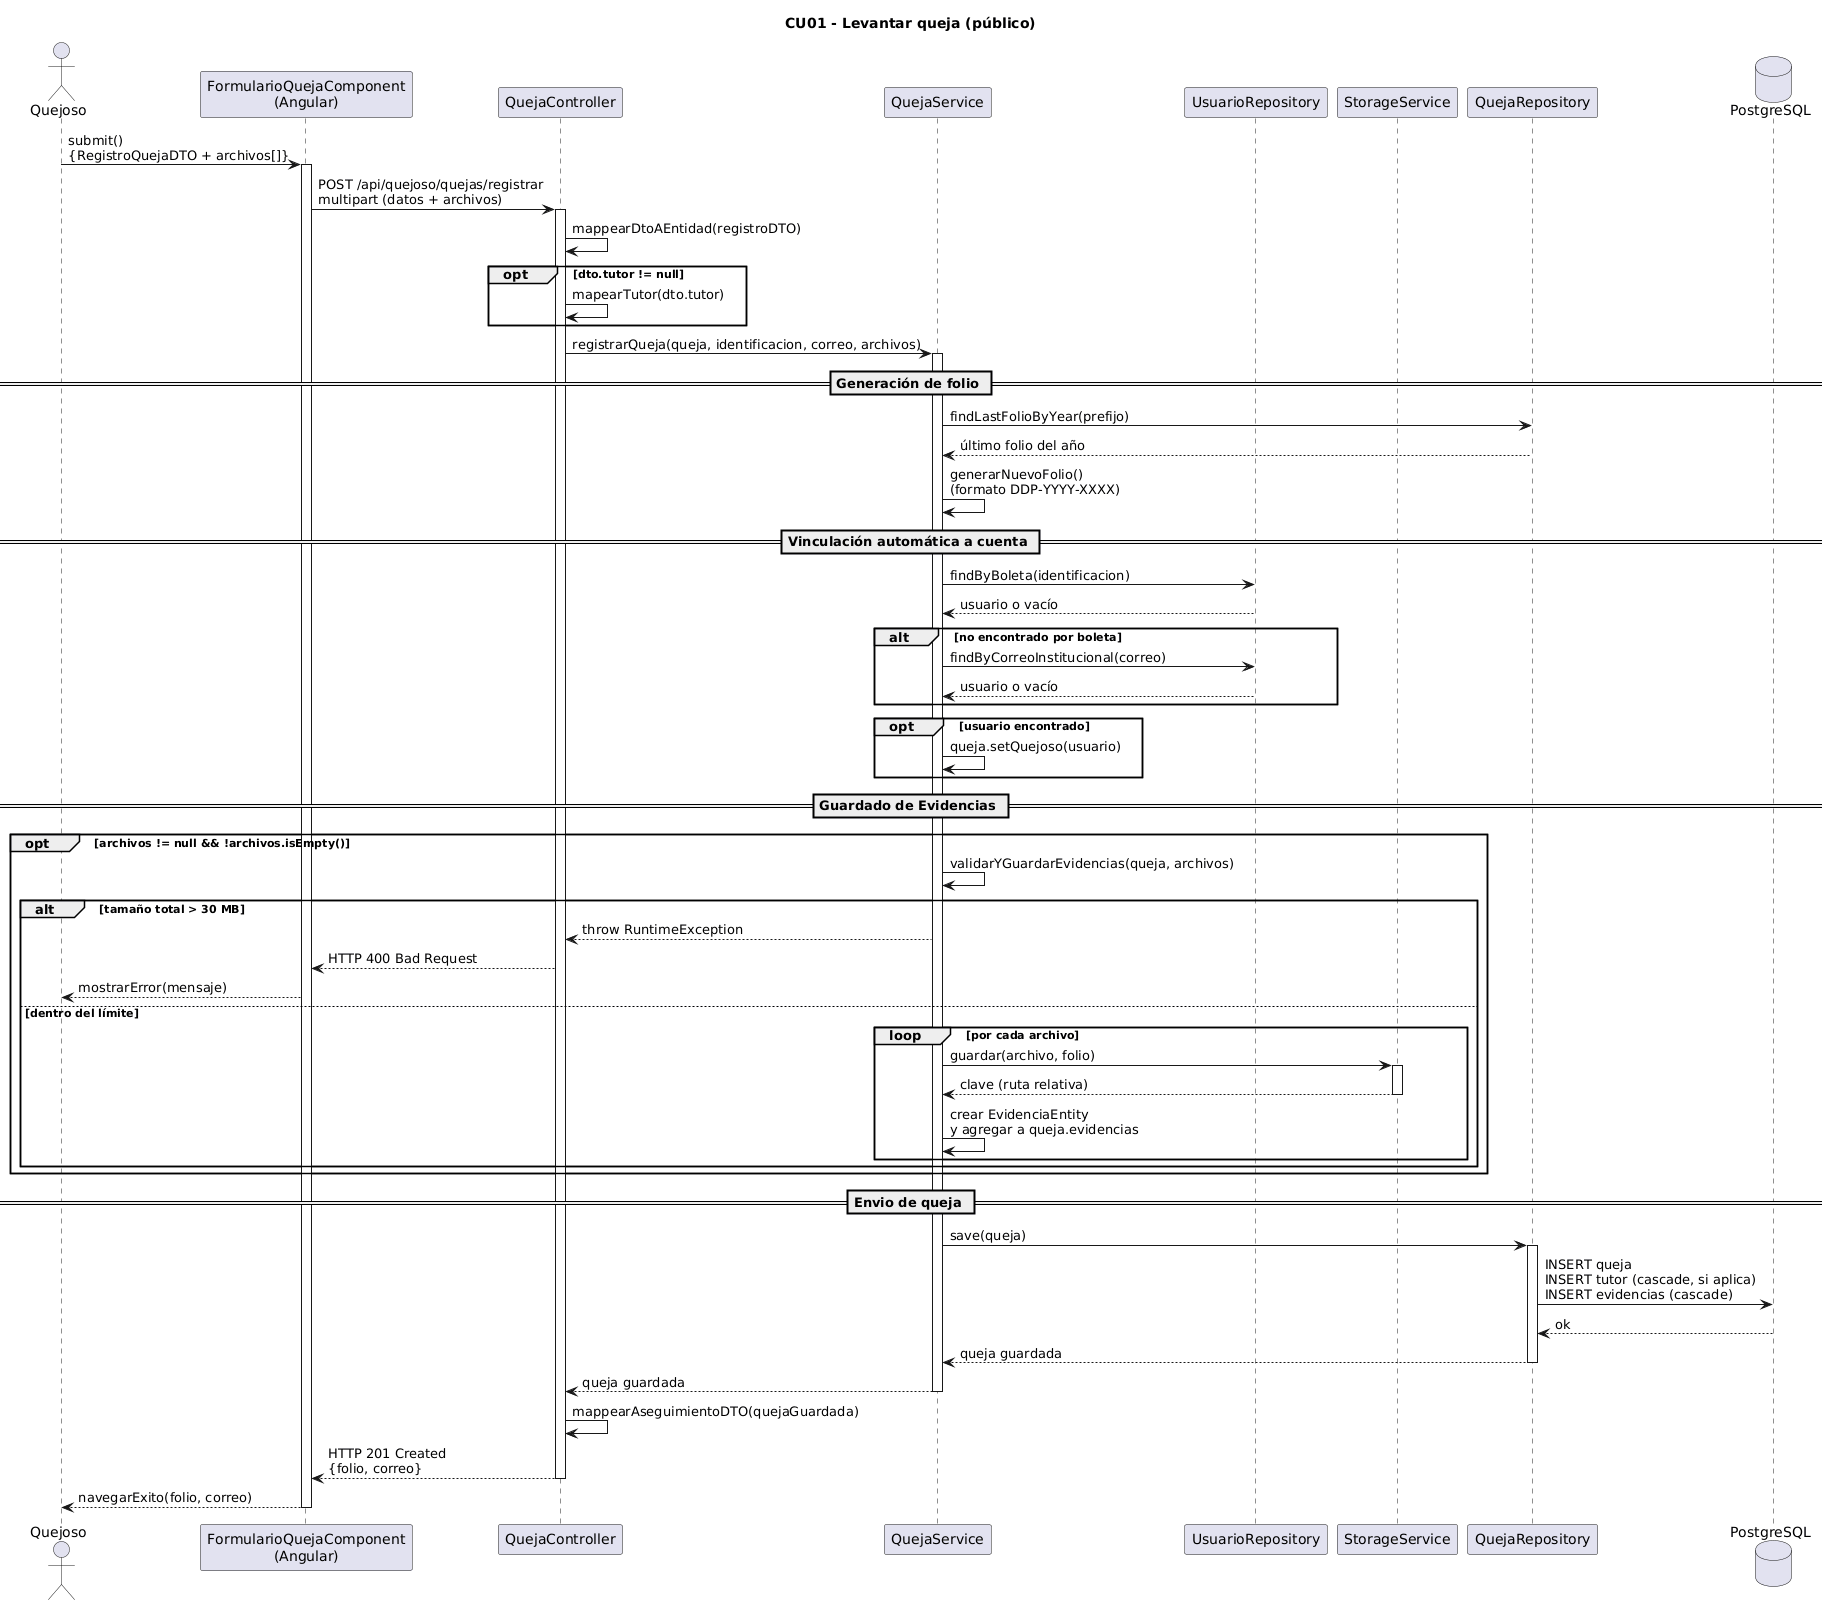
\includegraphics[width=0.90\textwidth, height=0.80\textheight, keepaspectratio]{imagenes/quejoso/D_Secuencia/CU01-LevantarQueja.png}
        \caption{Diagrama de Secuencia CU01: Levantar Queja}
        \label{fig:ds_cu01_levantar_queja}
    \end{figure}

    \clearpage

    % ---- CU03a ----
    \subsubsection{CU03: Crear Cuenta (Inicio)}

    Representa el inicio del flujo de creación de cuenta para un quejoso que ya cuenta con un folio asignado. El diagrama muestra la validación del folio y del correo electrónico en el sistema, así como la verificación de que no exista una cuenta activa previamente registrada con esos datos.

    \begin{figure}[H]
        \centering
        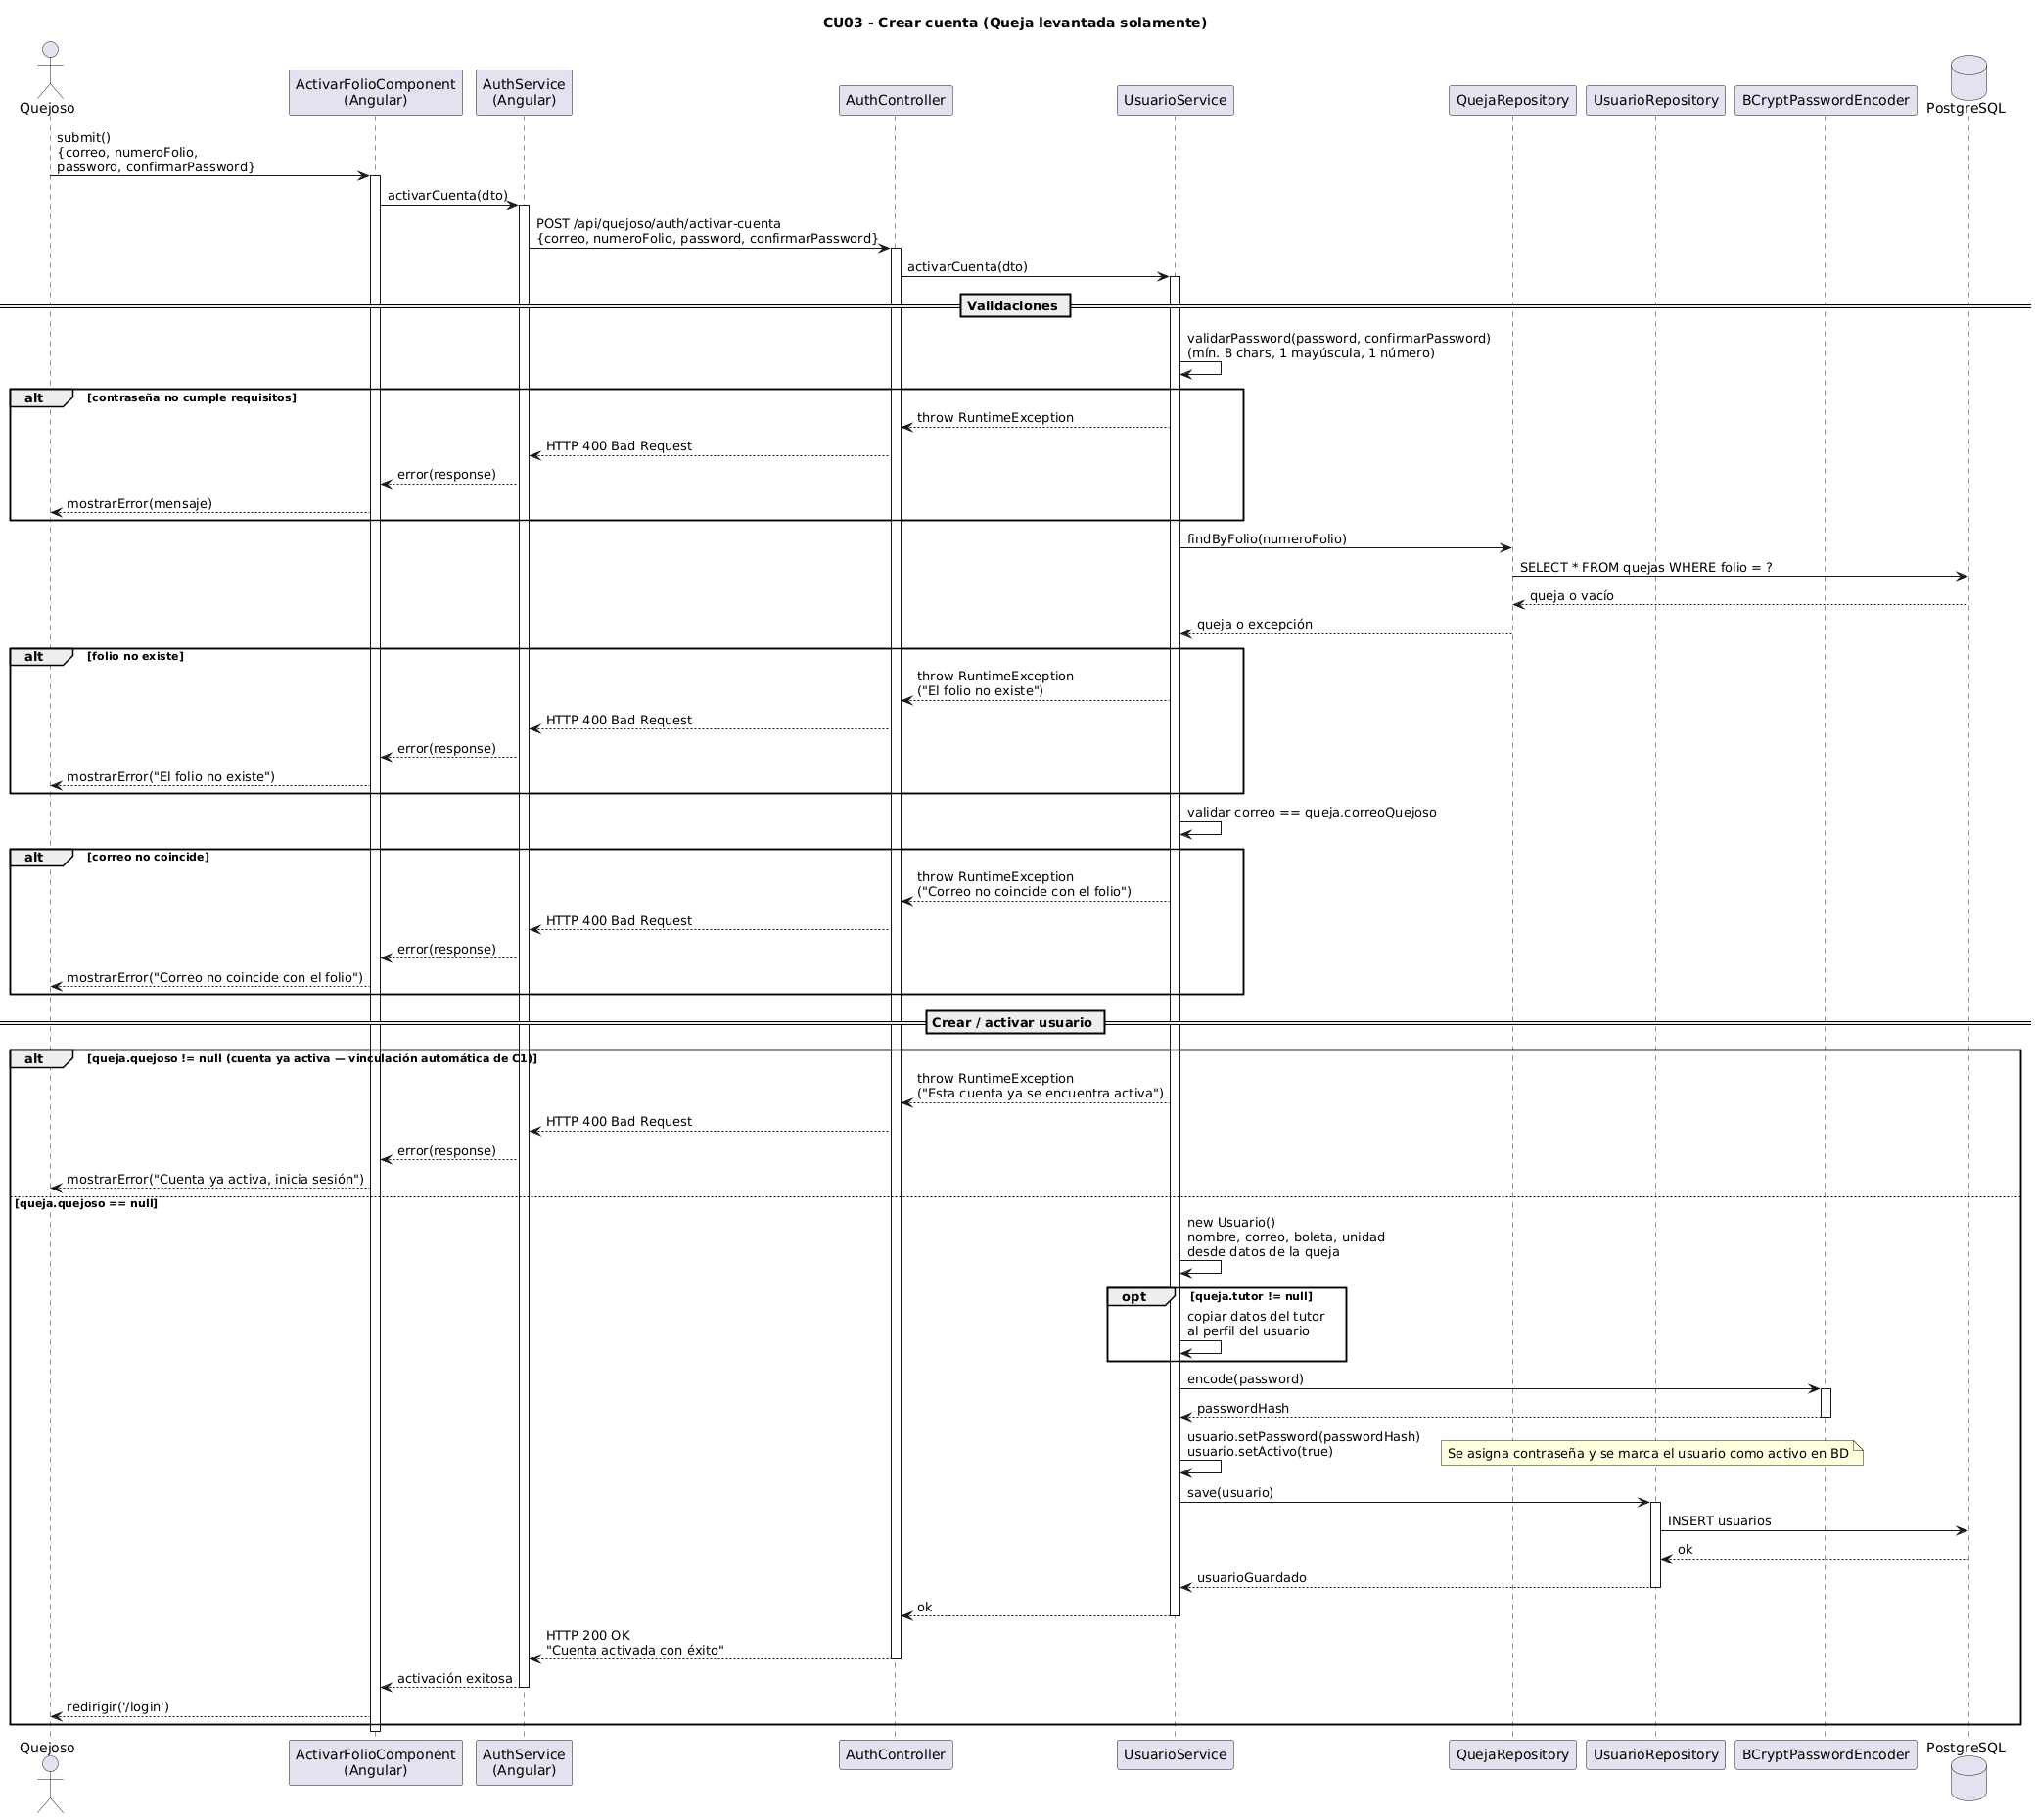
\includegraphics[width=0.90\textwidth, height=0.80\textheight, keepaspectratio]{imagenes/quejoso/D_Secuencia/CU03b-CrearCuenta(Inicio).png}
        \caption{Diagrama de Secuencia CU03: Crear Cuenta (Inicio)}
        \label{fig:ds_cu03a_crear_cuenta_inicio}
    \end{figure}

    \clearpage

    % ---- CU03b ----
    \subsubsection{CU03: Crear Cuenta (Éxito)}

    Representa el flujo de creacion de una cuenta pero cuando el quejoso levanta una queja, una vez superadas las validaciones. Describe la secuencia de mensajes para el establecimiento de la contraseña, el almacenamiento seguro de las credenciales y la notificación de activación exitosa de la cuenta, habilitando el acceso al dashboard del quejoso.

    \begin{figure}[H]
        \centering
        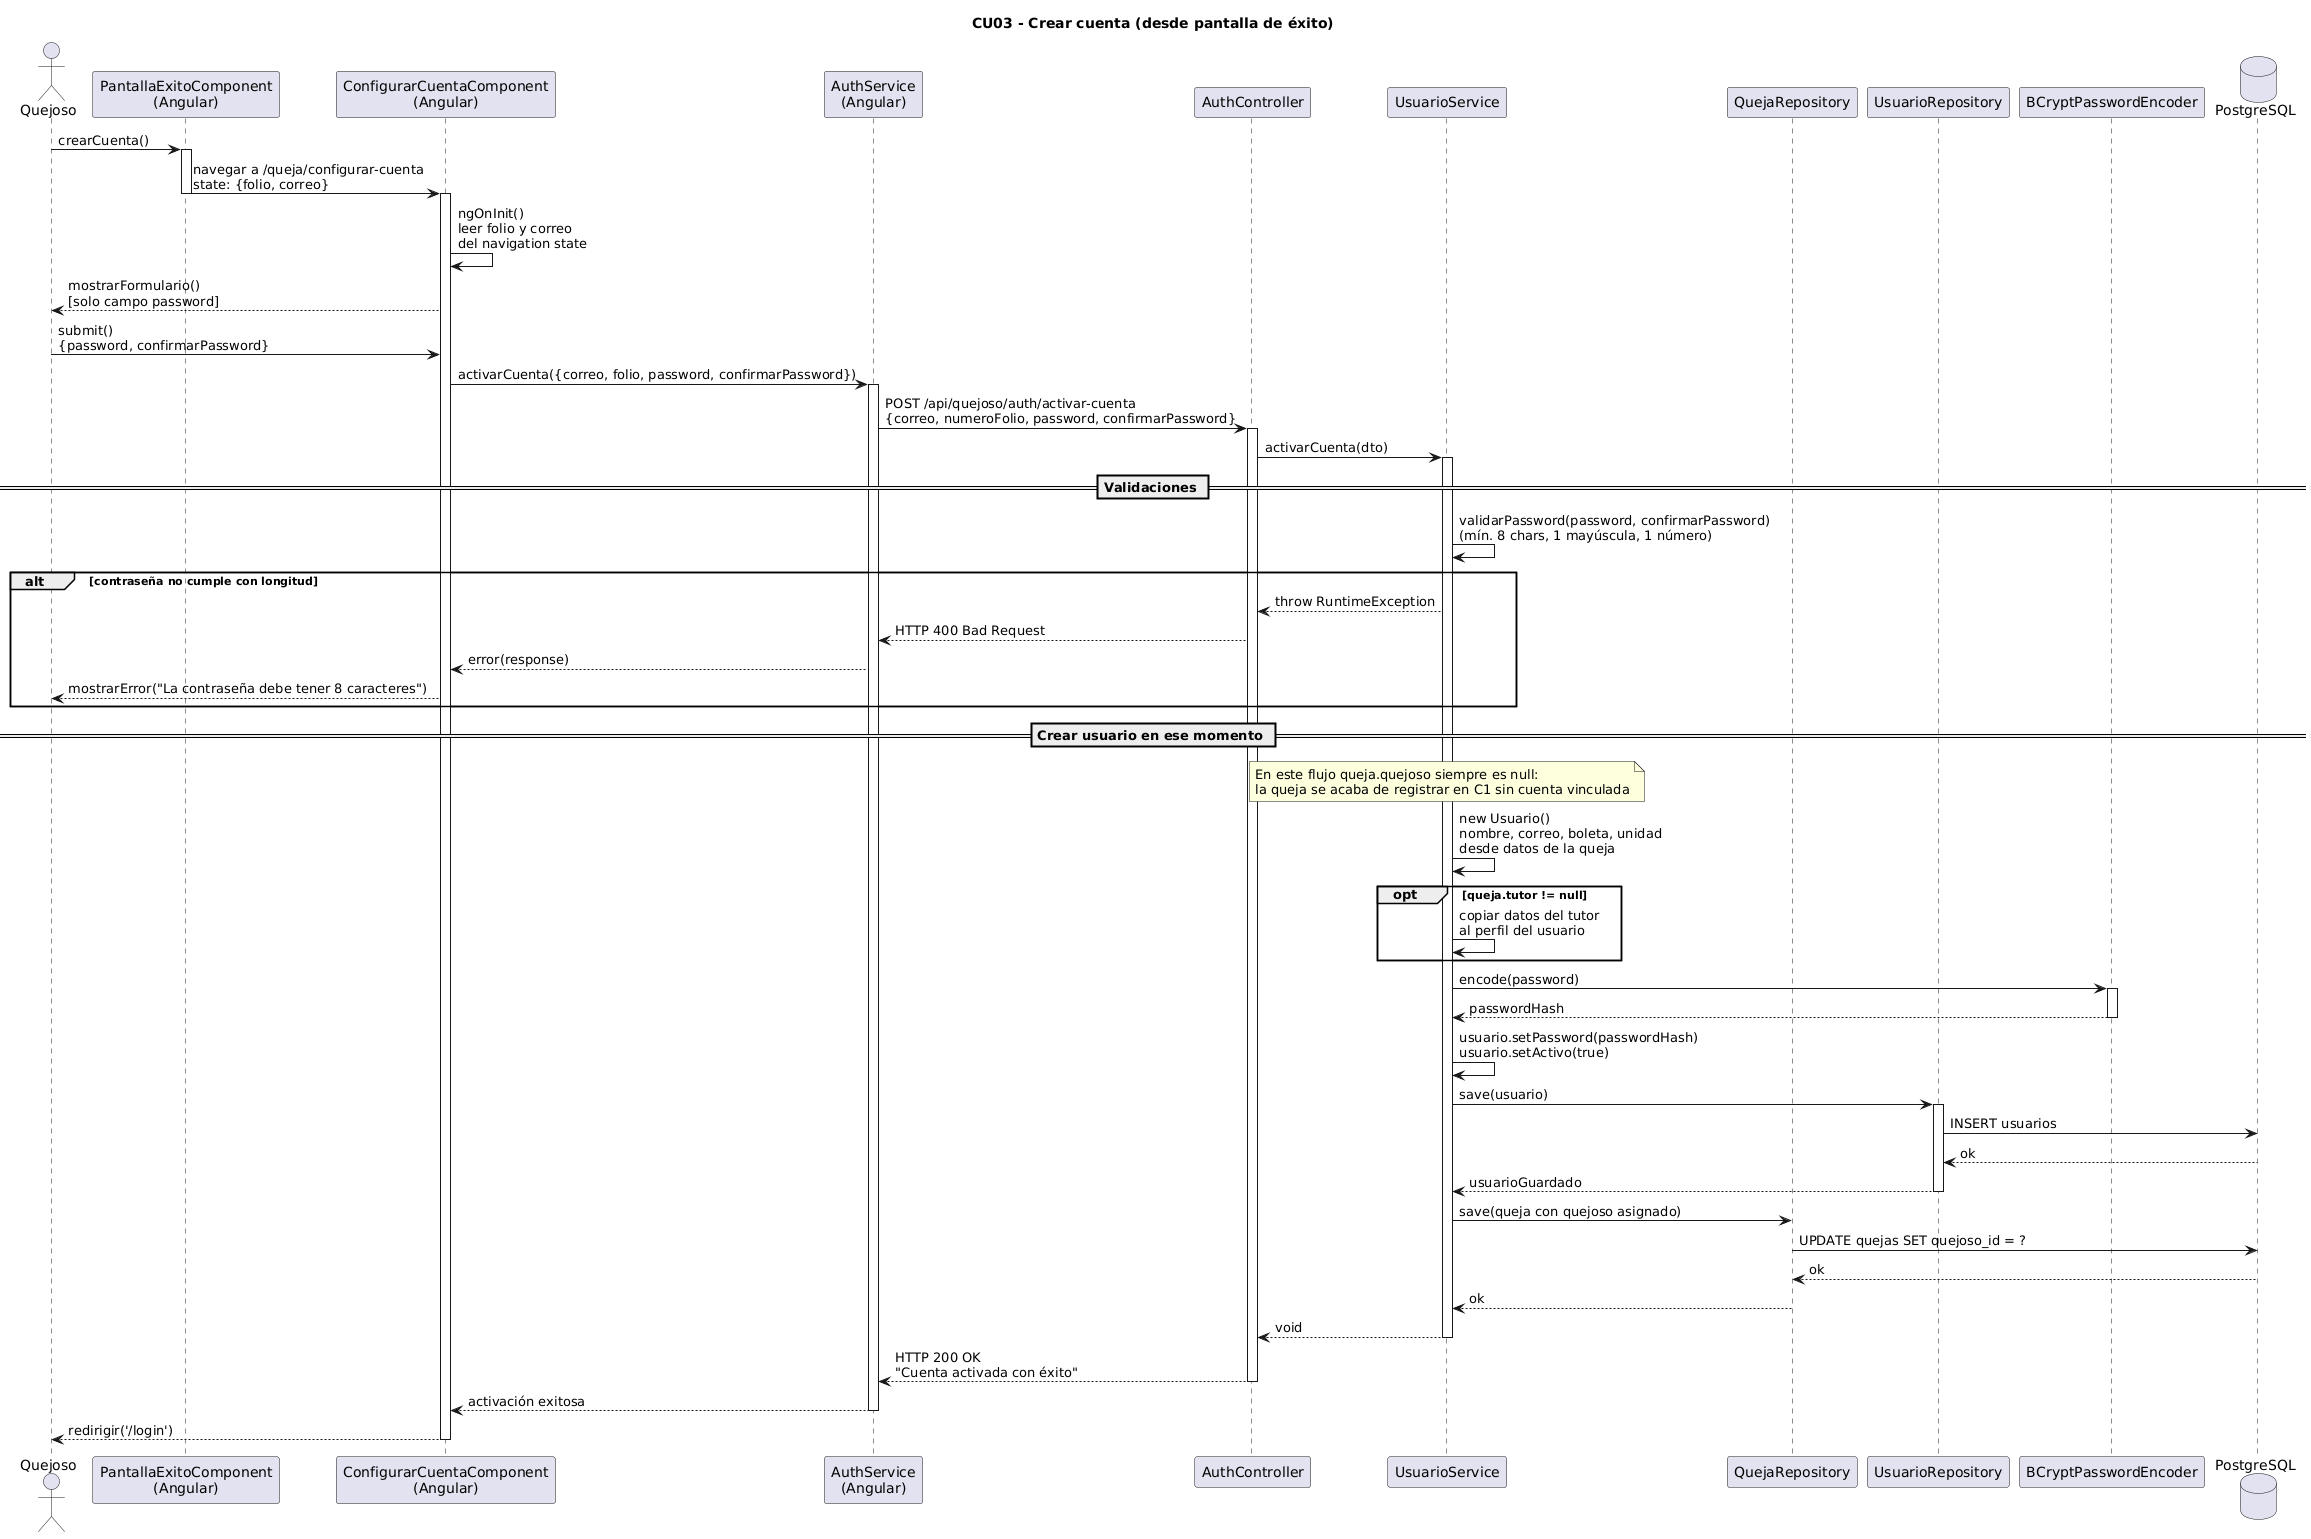
\includegraphics[width=0.90\textwidth, height=0.80\textheight, keepaspectratio]{imagenes/quejoso/D_Secuencia/CU03a-CrearCuenta(Exito).png}
        \caption{Diagrama de Secuencia CU03: Crear Cuenta (Éxito)}
        \label{fig:ds_cu03b_crear_cuenta_exito}
    \end{figure}

    \clearpage

    % ---- CU04 ----
    \subsubsection{CU04: Descarga de Acuse}

    Ilustra la secuencia para la descarga del acuse de recibo en formato PDF. El flujo muestra la solicitud del documento por parte del quejoso, la recuperación de los datos del folio desde el backend y la generación dinámica del archivo PDF para su descarga en el dispositivo del usuario.

    \begin{figure}[H]
        \centering
        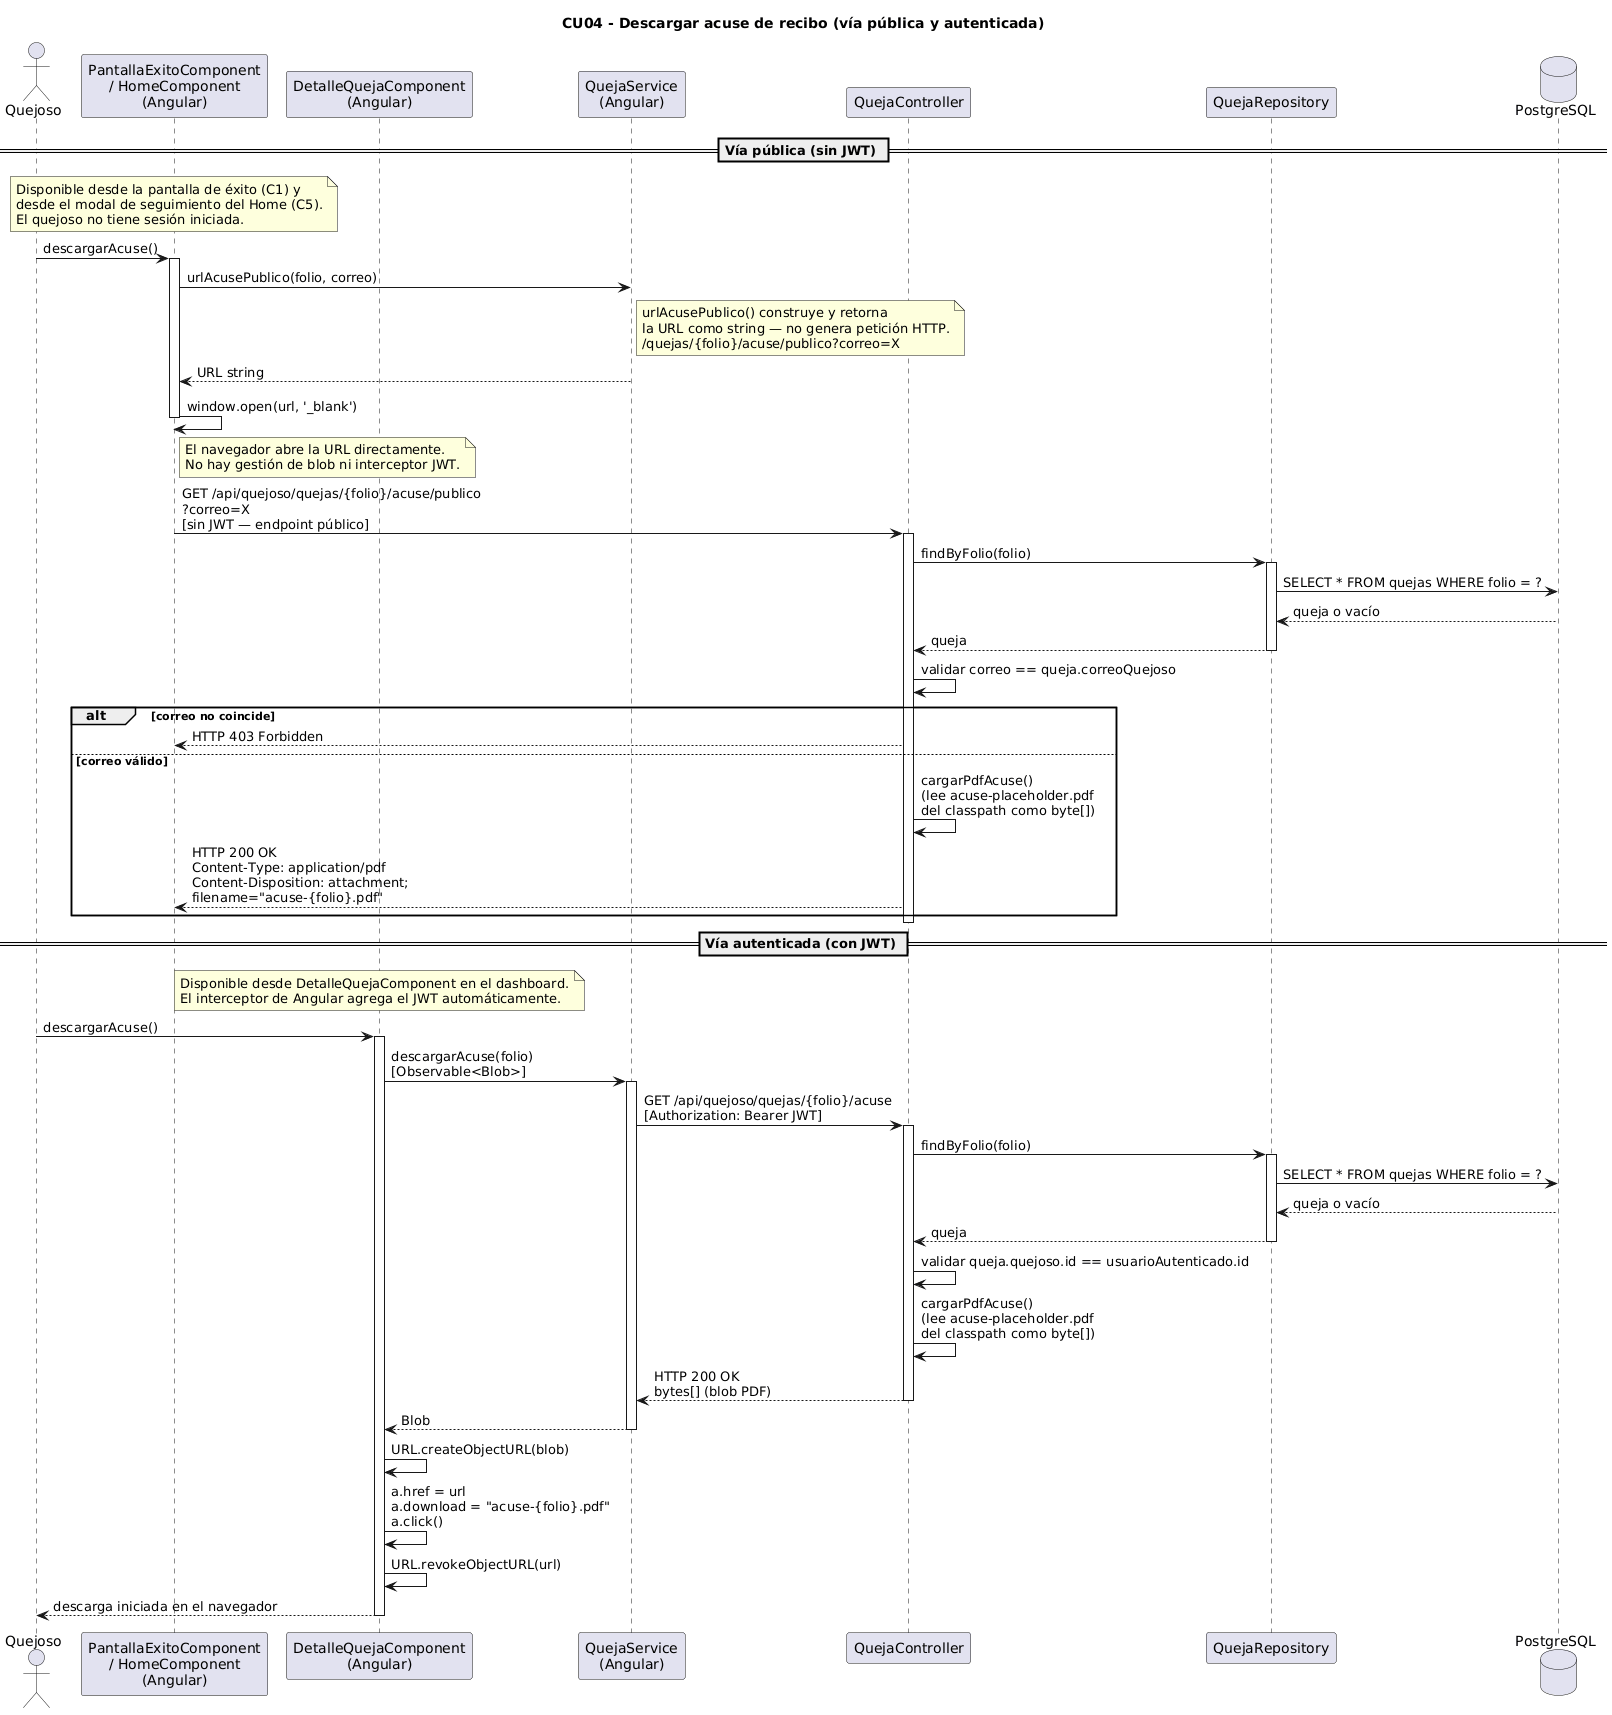
\includegraphics[width=0.90\textwidth, height=0.80\textheight, keepaspectratio]{imagenes/quejoso/D_Secuencia/CU04-DescargaAcuse.png}
        \caption{Diagrama de Secuencia CU04: Descarga de Acuse}
        \label{fig:ds_cu04_descarga_acuse}
    \end{figure}

    \clearpage

    % ---- CU05 ----
    \subsubsection{CU05: Detalle de Queja como Invitado}

    Describe el flujo que permite a un usuario sin cuenta activa consultar el estado de su trámite. El diagrama muestra la validación del folio y correo como credenciales temporales, y la recuperación de la información del expediente para su presentación en modo de solo lectura.

    \begin{figure}[H]
        \centering
        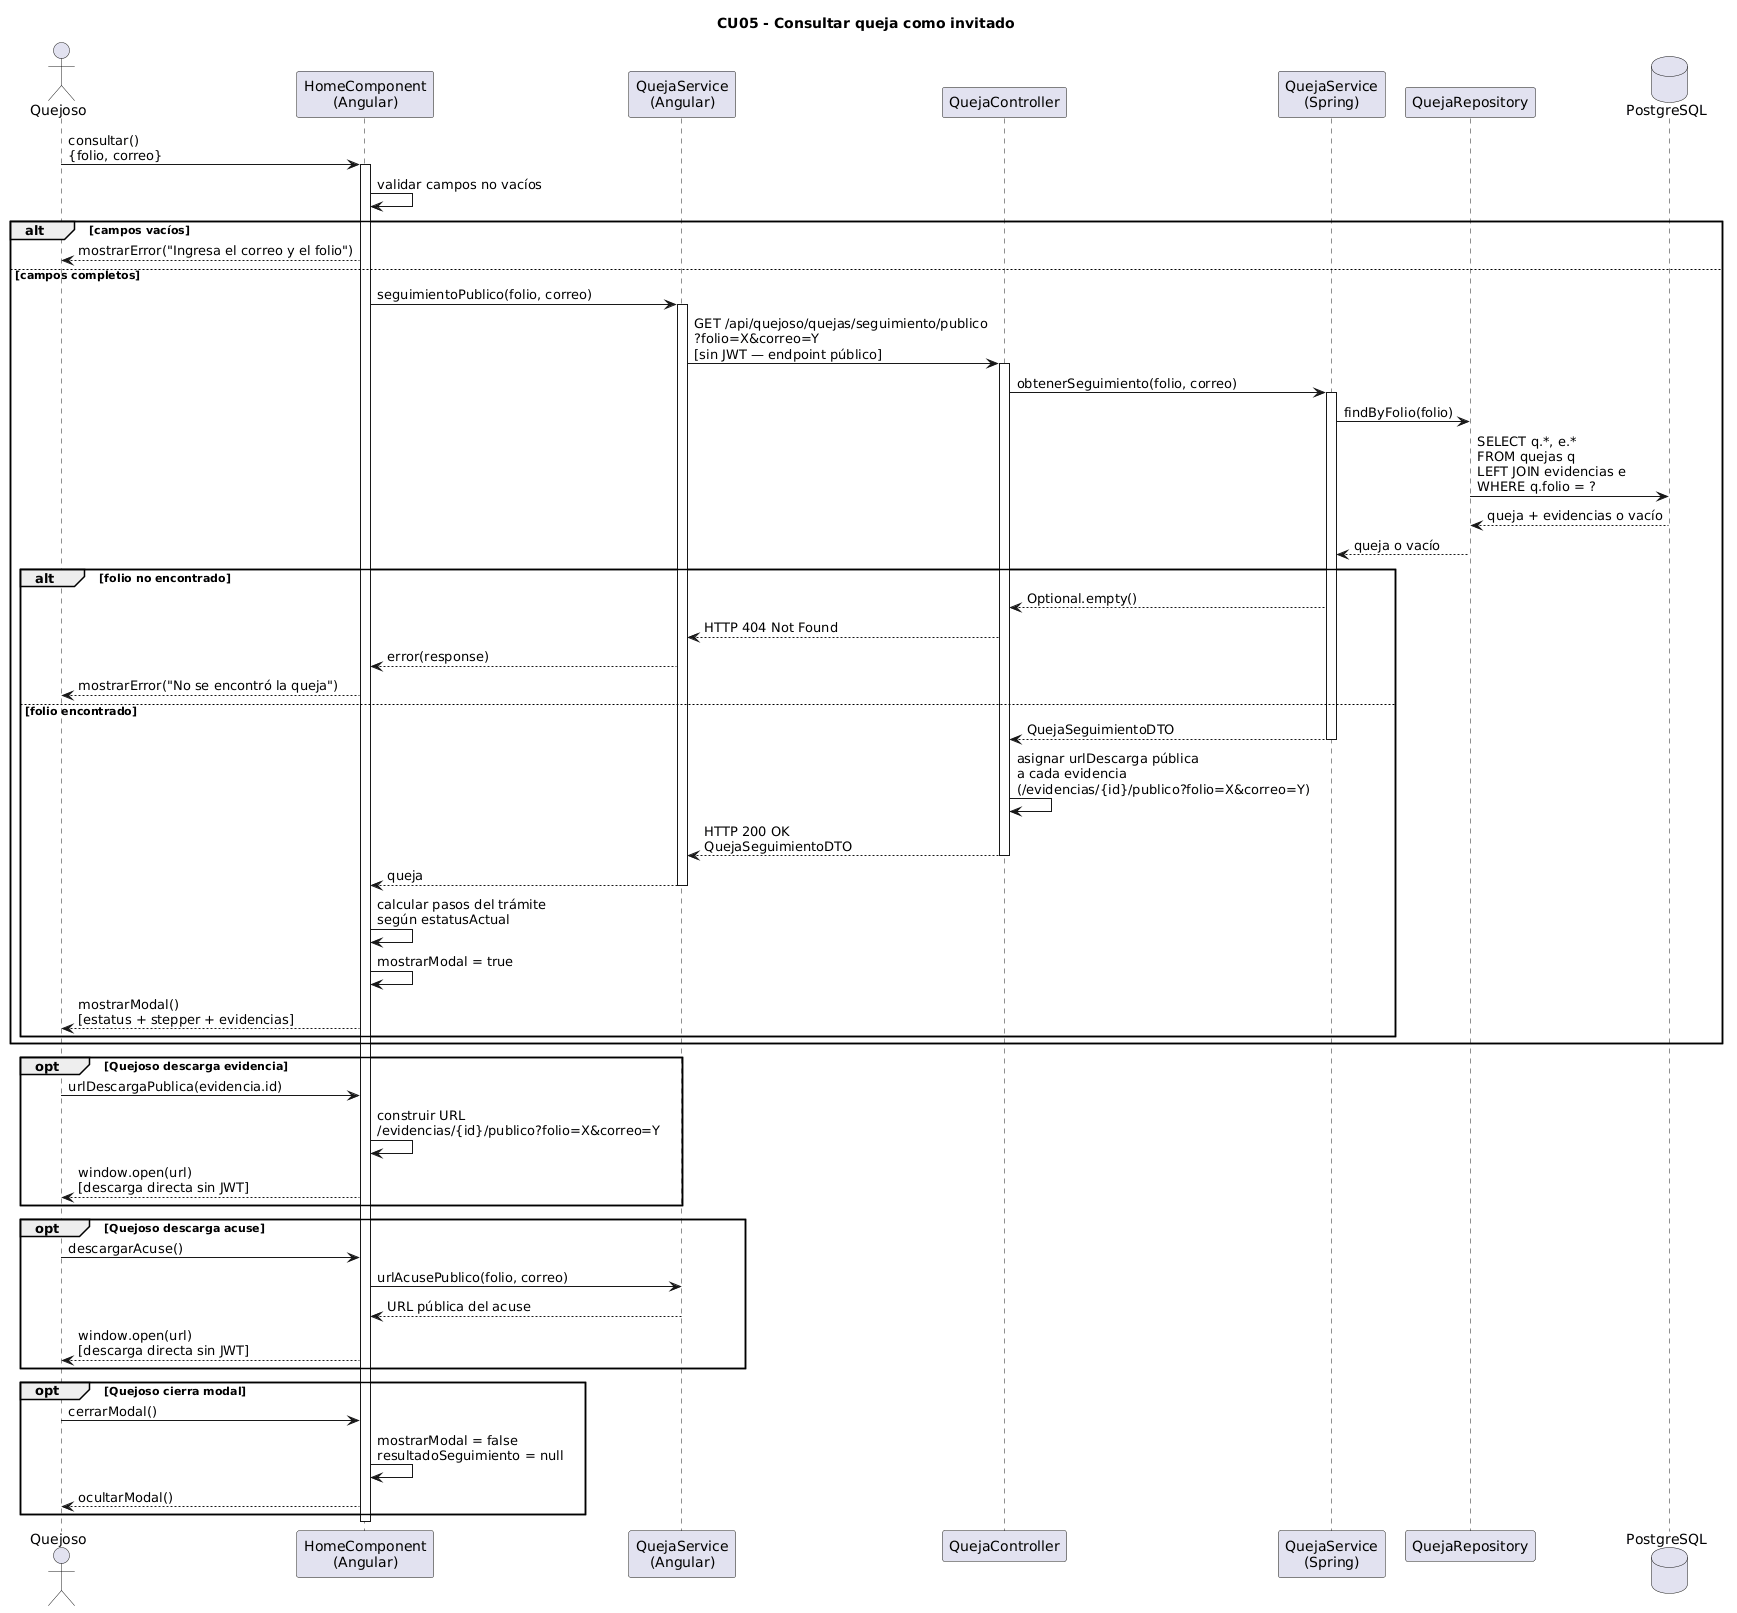
\includegraphics[width=0.90\textwidth, height=0.80\textheight, keepaspectratio]{imagenes/quejoso/D_Secuencia/CU05-DetalleQuejaInvitado.png}
        \caption{Diagrama de Secuencia CU05: Detalle de Queja como Invitado}
        \label{fig:ds_cu05_detalle_queja_invitado}
    \end{figure}

    \clearpage

    % ---- CU06 ----
    \subsubsection{CU06: Iniciar Sesión}

    Representa la secuencia de autenticación del quejoso registrado. El flujo contempla la captura de credenciales, la verificación contra la base de datos, la generación del token de sesión y la redirección al dashboard principal en caso de autenticación exitosa, así como el manejo de errores ante credenciales inválidas.

    \begin{figure}[H]
        \centering
        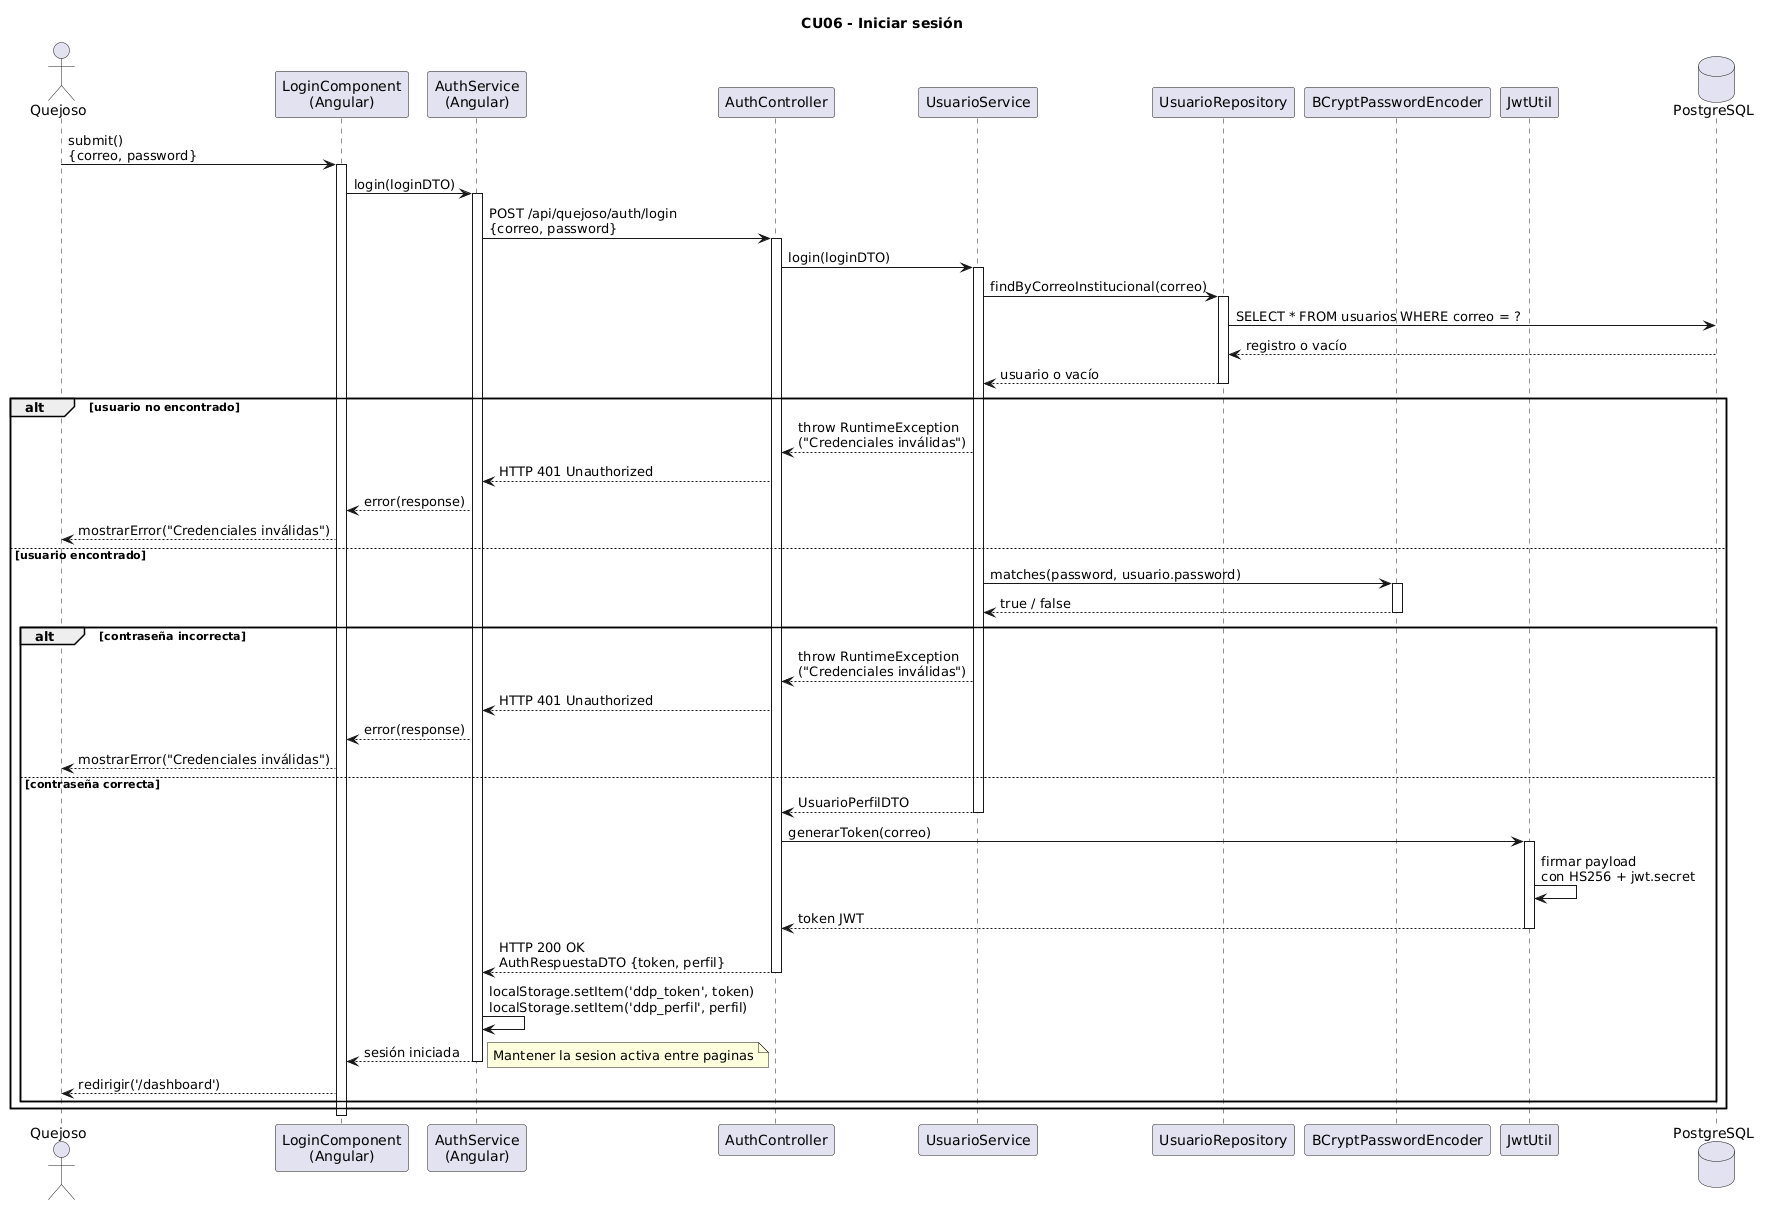
\includegraphics[width=0.90\textwidth, height=0.80\textheight, keepaspectratio]{imagenes/quejoso/D_Secuencia/CU06-IniciarSesion.png}
        \caption{Diagrama de Secuencia CU06: Iniciar Sesión}
        \label{fig:ds_cu06_iniciar_sesion}
    \end{figure}

    \clearpage

    % ---- CU07 ----
    \subsubsection{CU07: Recuperar Contraseña}

    Ilustra el flujo de recuperación de acceso para el quejoso que olvidó sus credenciales. El diagrama muestra la solicitud del enlace de restablecimiento mediante correo, la generación y envío del token de recuperación, y la secuencia de validación y actualización de la nueva contraseña en la base de datos.

    \begin{figure}[H]
        \centering
        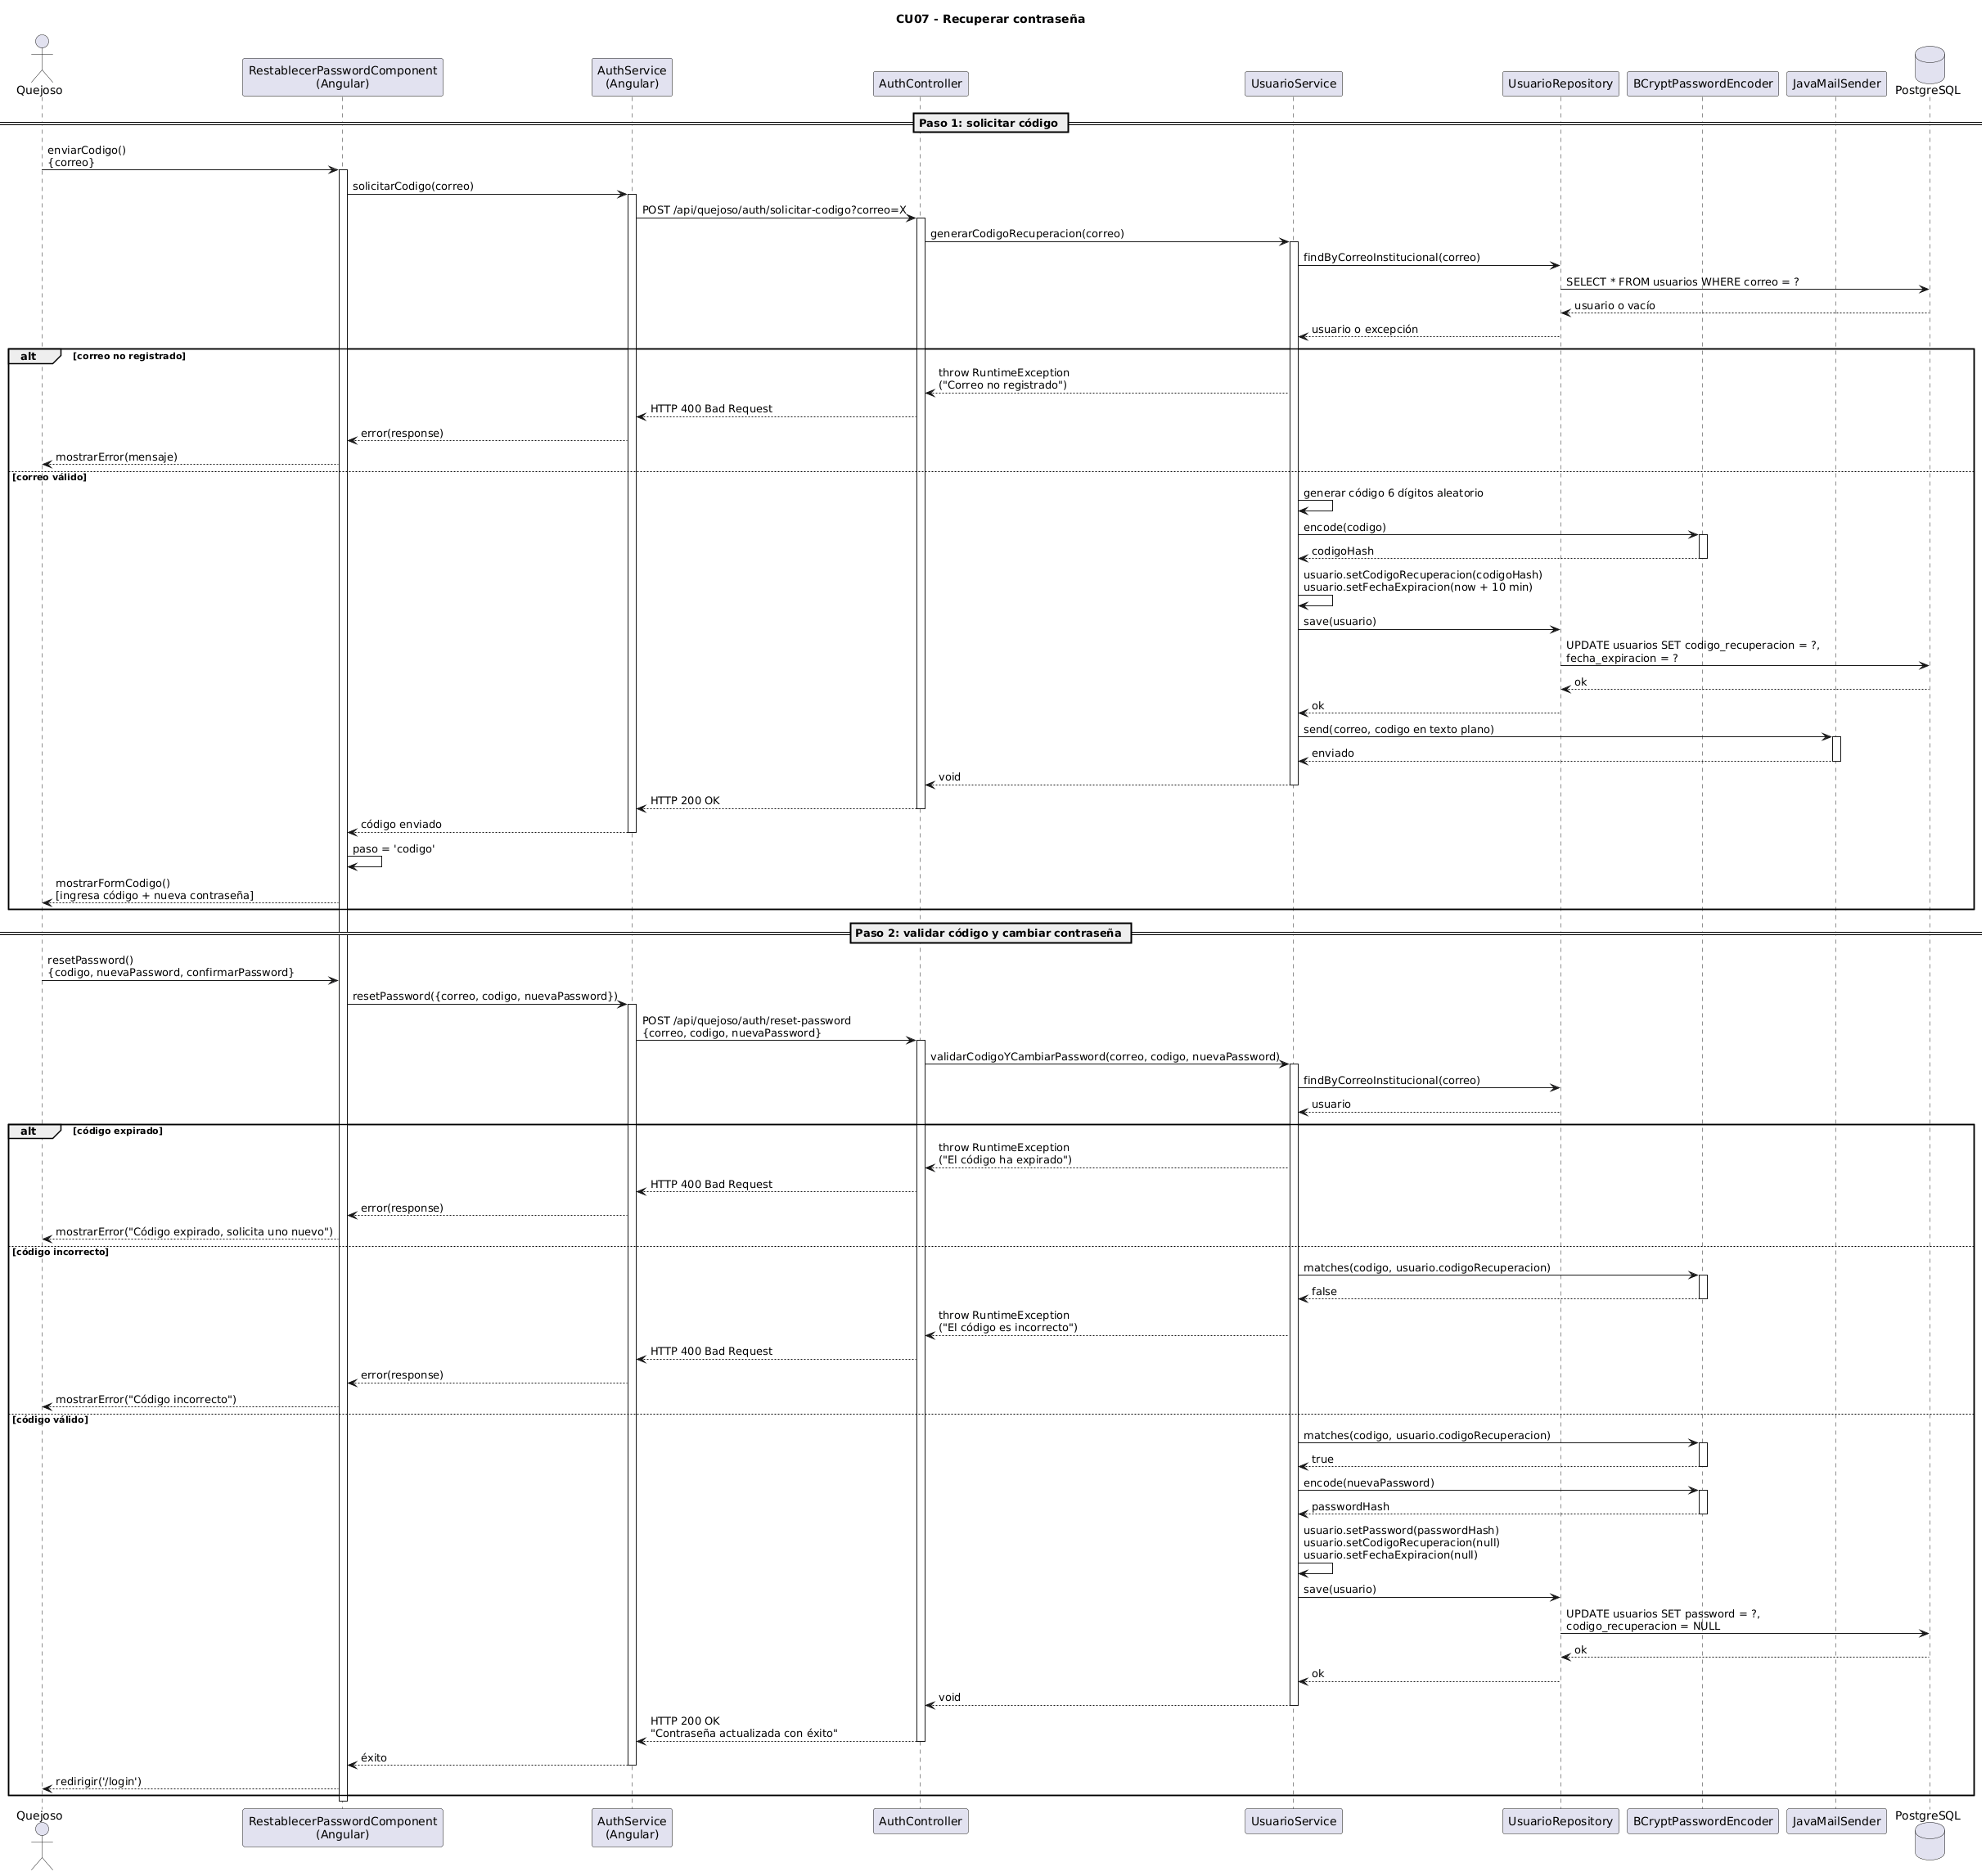
\includegraphics[width=0.90\textwidth, height=0.80\textheight, keepaspectratio]{imagenes/quejoso/D_Secuencia/CU07-RecuperarContraseña.png}
        \caption{Diagrama de Secuencia CU07: Recuperar Contraseña}
        \label{fig:ds_cu07_recuperar_contrasena}
    \end{figure}

    \clearpage

    % ---- CU08 ----
    \subsubsection{CU08: Dashboard Resumen}

    Describe la secuencia de carga del panel principal del quejoso autenticado. El flujo muestra las consultas paralelas al backend para recuperar los contadores de estatus de quejas (Recibidas, En Revisión, Concluidas) y el listado de los trámites más recientes del usuario.

    \begin{figure}[H]
        \centering
        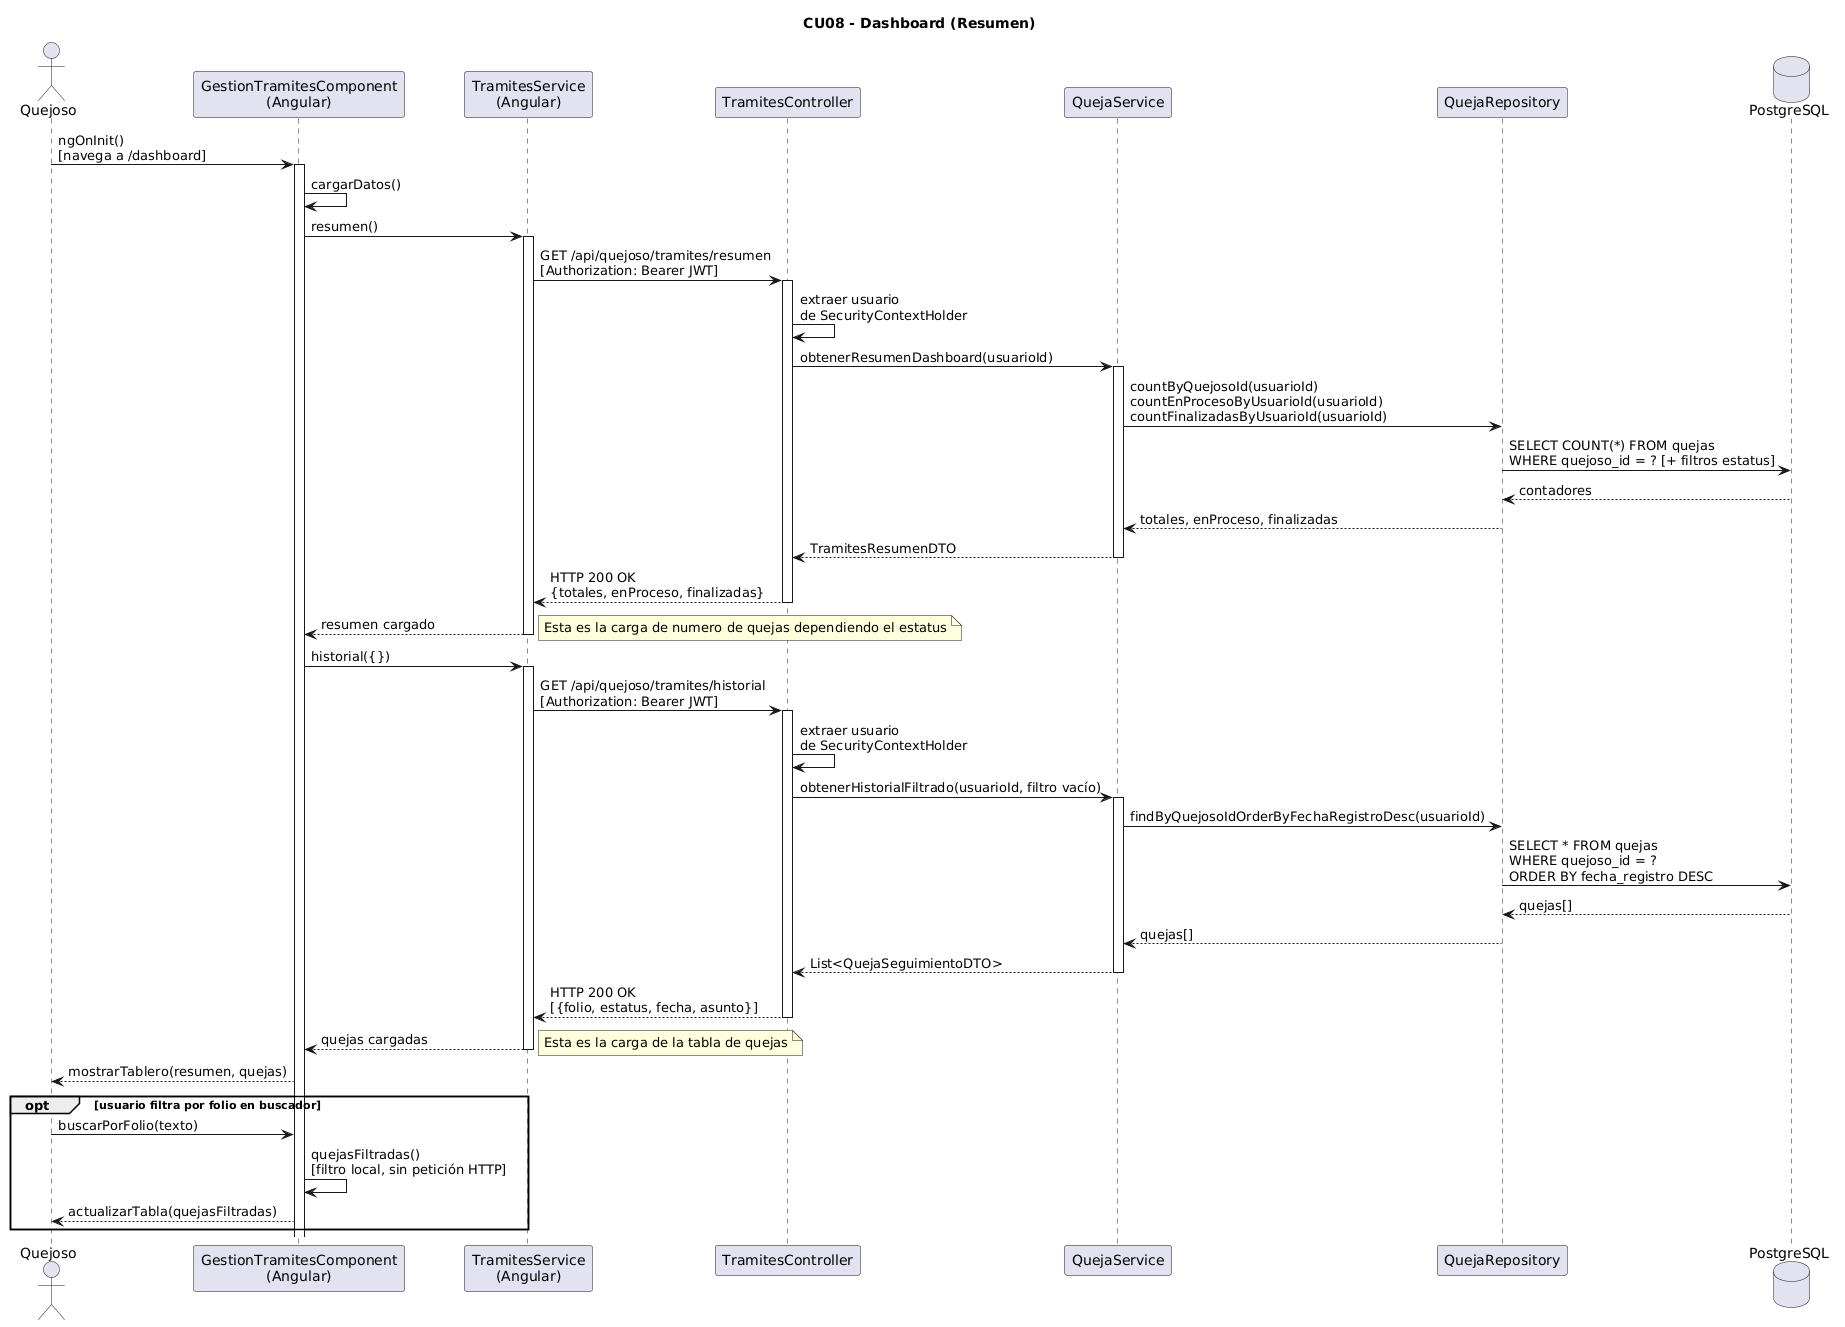
\includegraphics[width=0.90\textwidth, height=0.80\textheight, keepaspectratio]{imagenes/quejoso/D_Secuencia/CU08-DashboardResumen.png}
        \caption{Diagrama de Secuencia CU08: Dashboard Resumen}
        \label{fig:ds_cu08_dashboard_resumen}
    \end{figure}

    \clearpage

    % ---- CU09 ----
    \subsubsection{CU09: Modificar Queja}

    Representa la secuencia de edición de una queja existente. El diagrama contempla la recuperación de los datos actuales del expediente, la validación de que el estatus permita modificaciones (solo quejas en estado "RECIBIDA"), la actualización de la información en el backend y la confirmación del cambio al usuario.

    \begin{figure}[H]
        \centering
        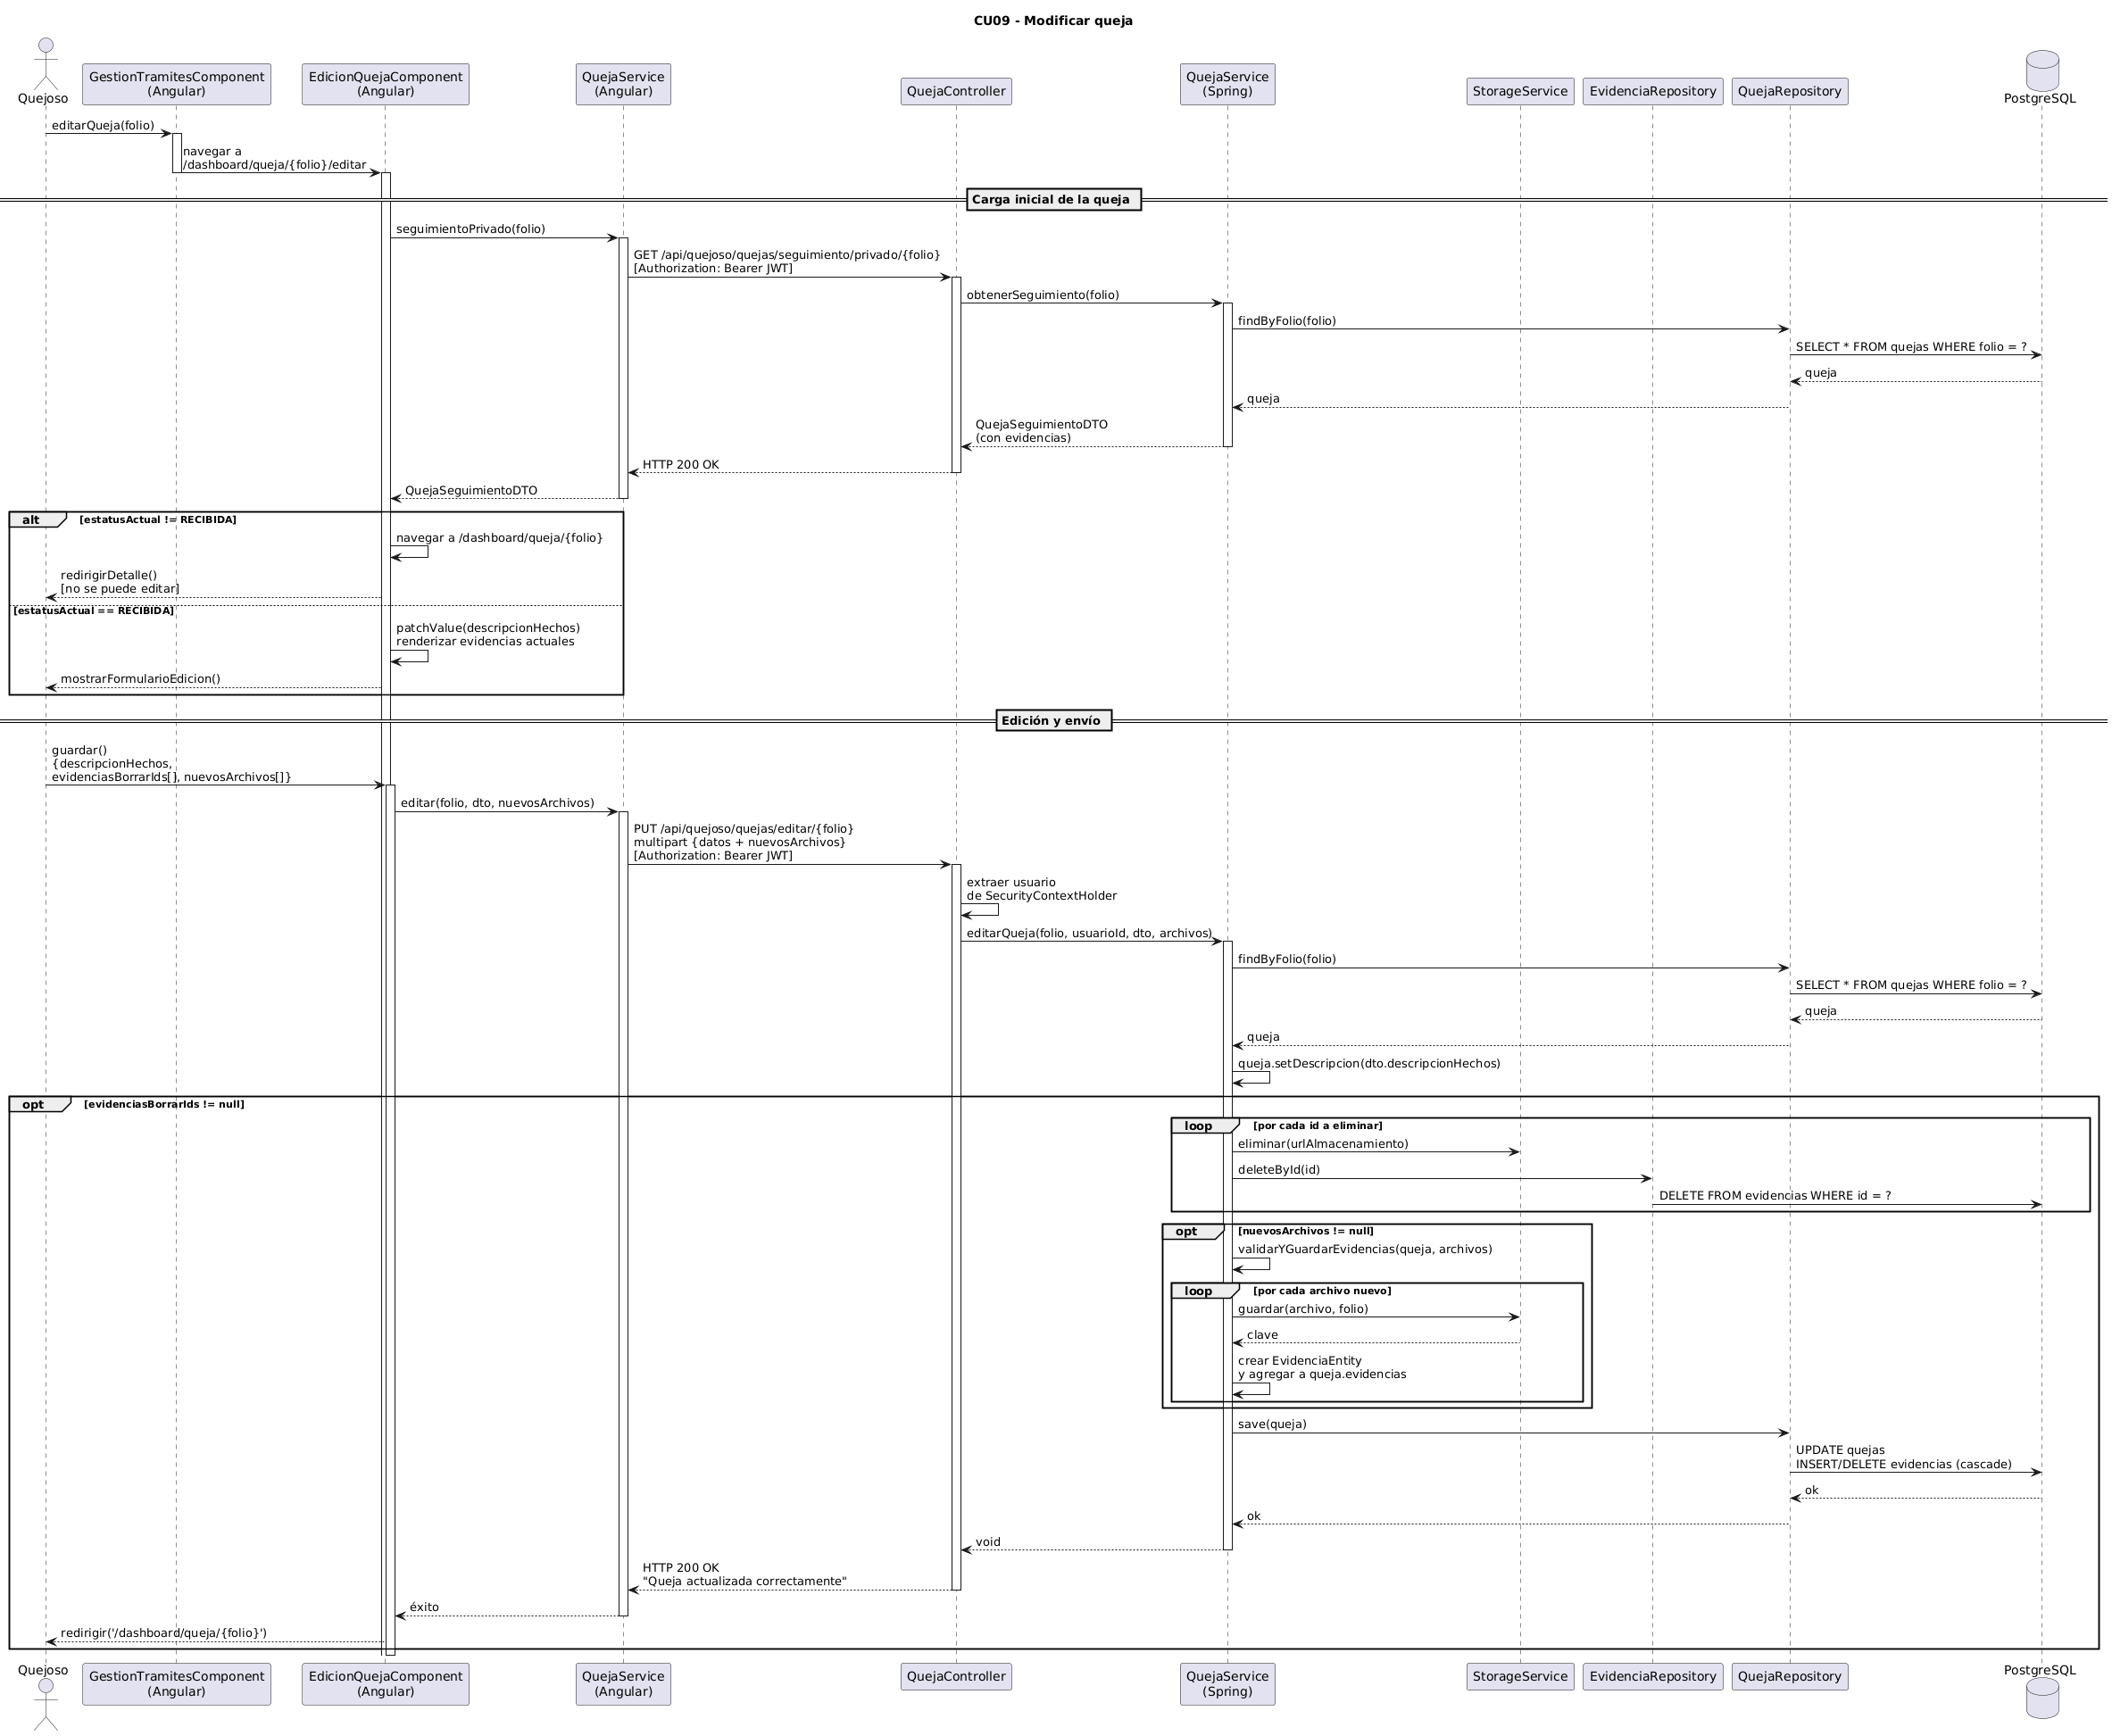
\includegraphics[width=0.90\textwidth, height=0.80\textheight, keepaspectratio]{imagenes/quejoso/D_Secuencia/CU09-ModificarQueja.png}
        \caption{Diagrama de Secuencia CU09: Modificar Queja}
        \label{fig:ds_cu09_modificar_queja}
    \end{figure}

    \clearpage

    % ---- CU11 ----
    \subsubsection{CU11: Eliminar Queja}

    Ilustra el flujo de cancelación lógica de una queja. El diagrama muestra la validación del estatus de la queja como condición previa, la presentación del diálogo de confirmación al usuario y la ejecución de la eliminación lógica en la base de datos sin borrado físico del registro.

    \begin{figure}[H]
        \centering
        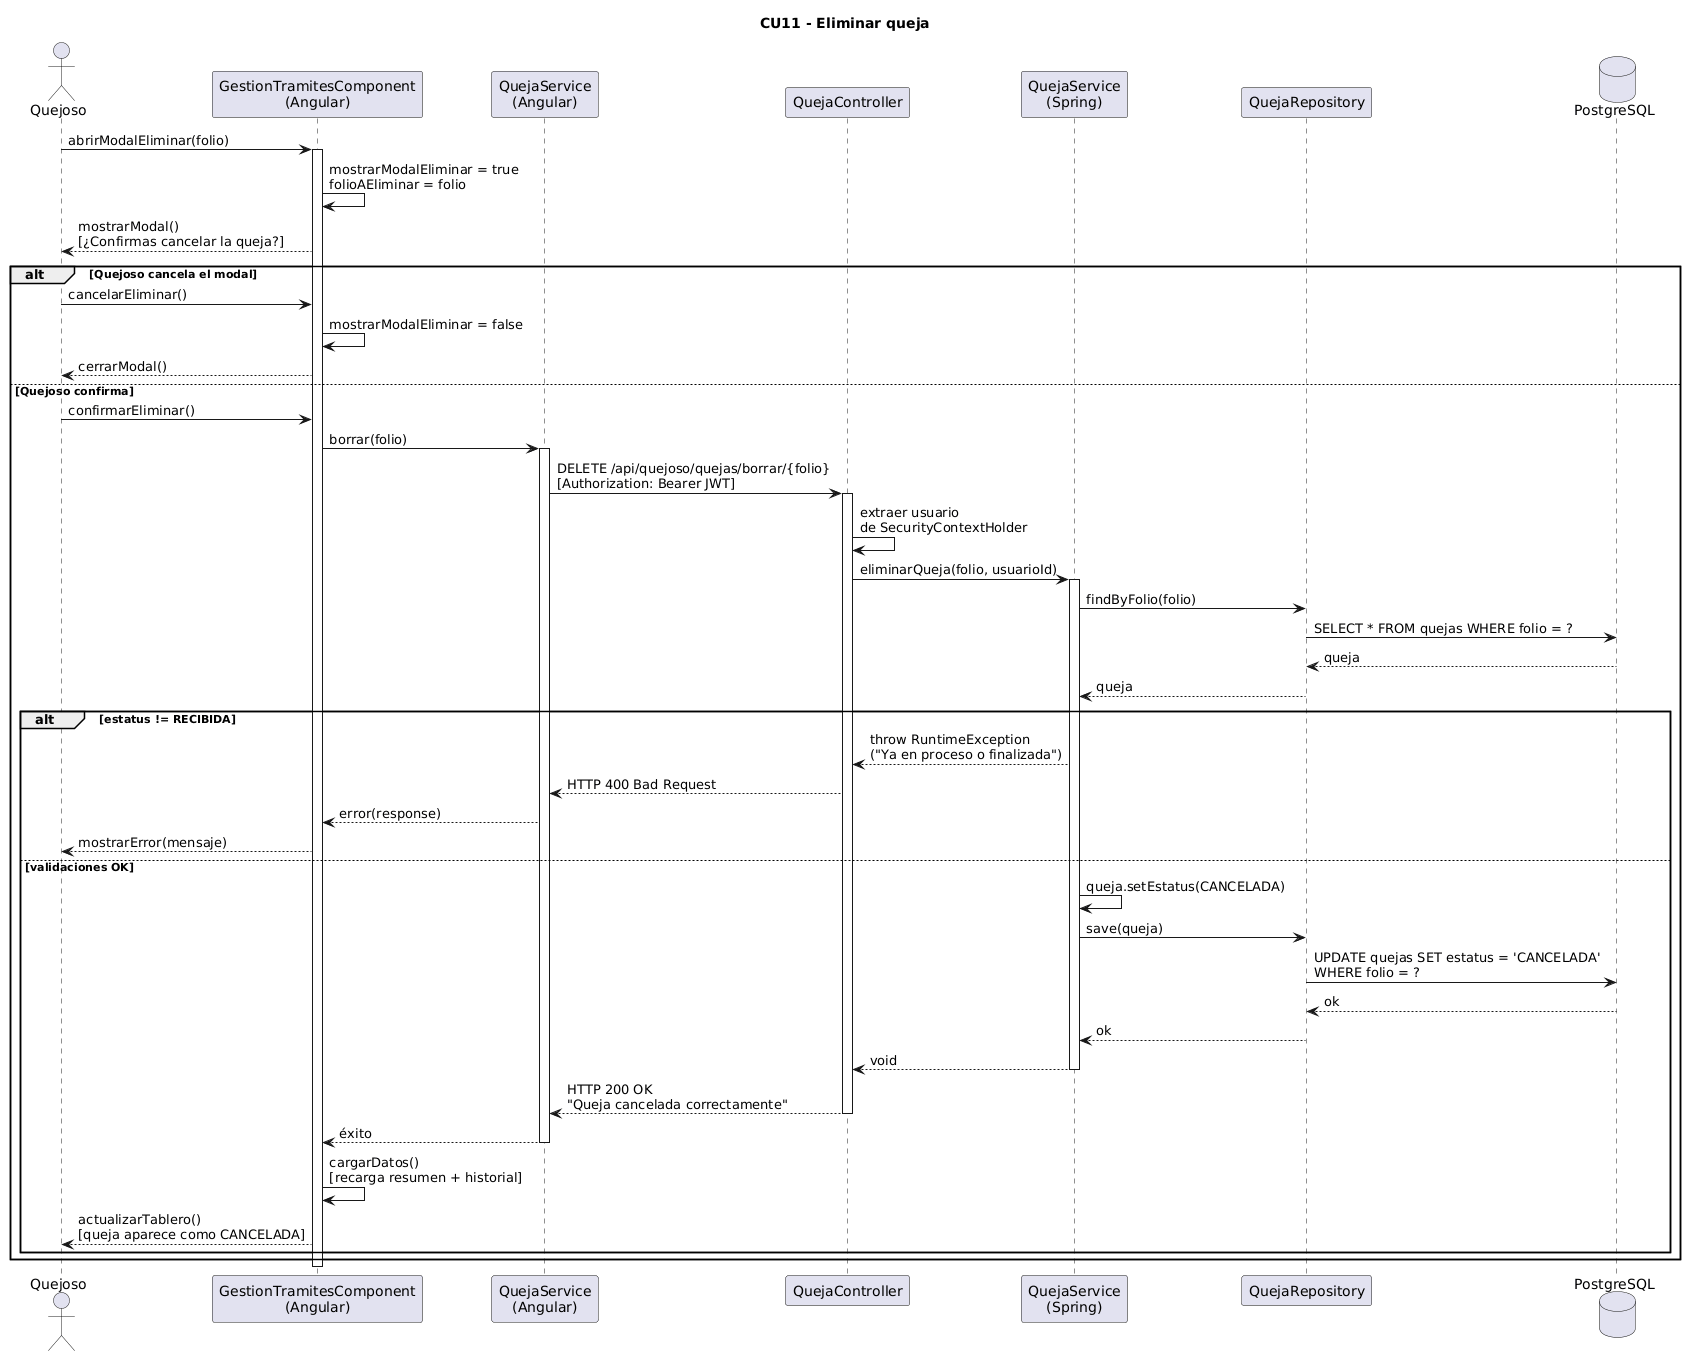
\includegraphics[width=0.90\textwidth, height=0.80\textheight, keepaspectratio]{imagenes/quejoso/D_Secuencia/CU11-EliminarQueja.png}
        \caption{Diagrama de Secuencia CU11: Eliminar Queja}
        \label{fig:ds_cu11_eliminar_queja}
    \end{figure}

    \clearpage

    % ---- CU12 ----
    \subsubsection{CU12: Detalle de Queja}

    Describe la secuencia de consulta del detalle de un expediente por parte del quejoso autenticado. El flujo contempla la recuperación de los campos del folio (datos del solicitante, cronología de estatus, narrativa y archivos adjuntos) y su presentación en la interfaz de detalle.

    \begin{figure}[H]
        \centering
        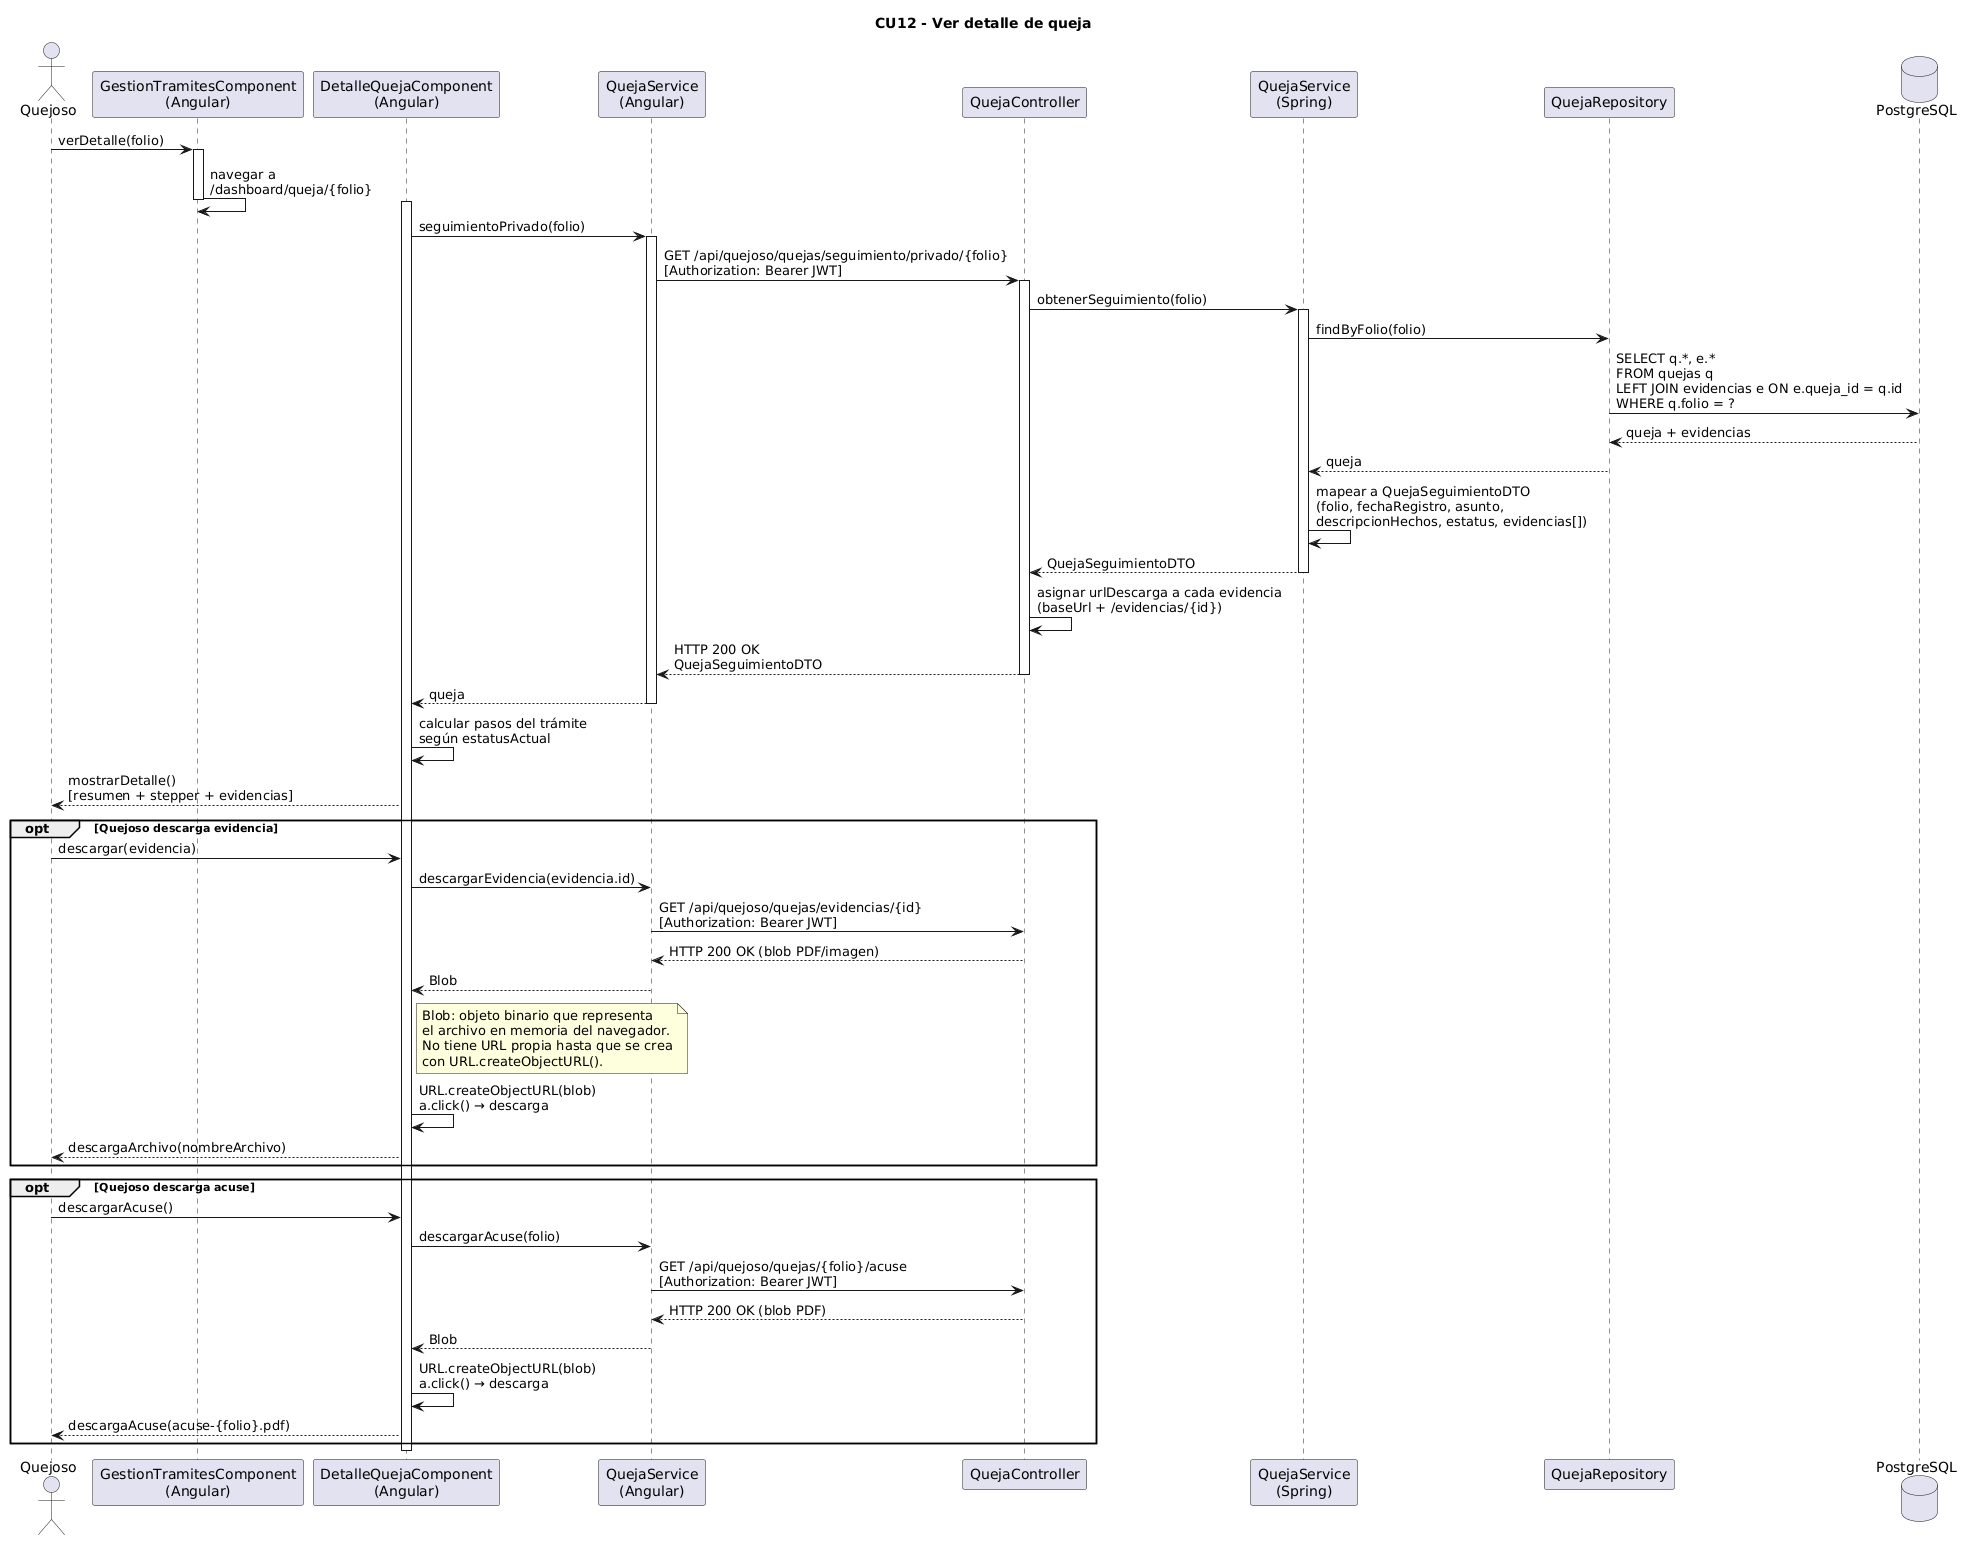
\includegraphics[width=0.90\textwidth, height=0.80\textheight, keepaspectratio]{imagenes/quejoso/D_Secuencia/CU12-DetalleQueja.png}
        \caption{Diagrama de Secuencia CU12: Detalle de Queja}
        \label{fig:ds_cu12_detalle_queja}
    \end{figure}

    \clearpage

    % ---- CU13 ----
    \subsubsection{CU13: Historial de Quejas}

    Representa el flujo de consulta del historial completo de trámites del usuario. El diagrama muestra la solicitud al backend con parámetros de filtrado por estatus y fecha, la recuperación del listado y la presentación de los resultados en la tabla de historial con opción de descarga de acuses.

    \begin{figure}[H]
        \centering
        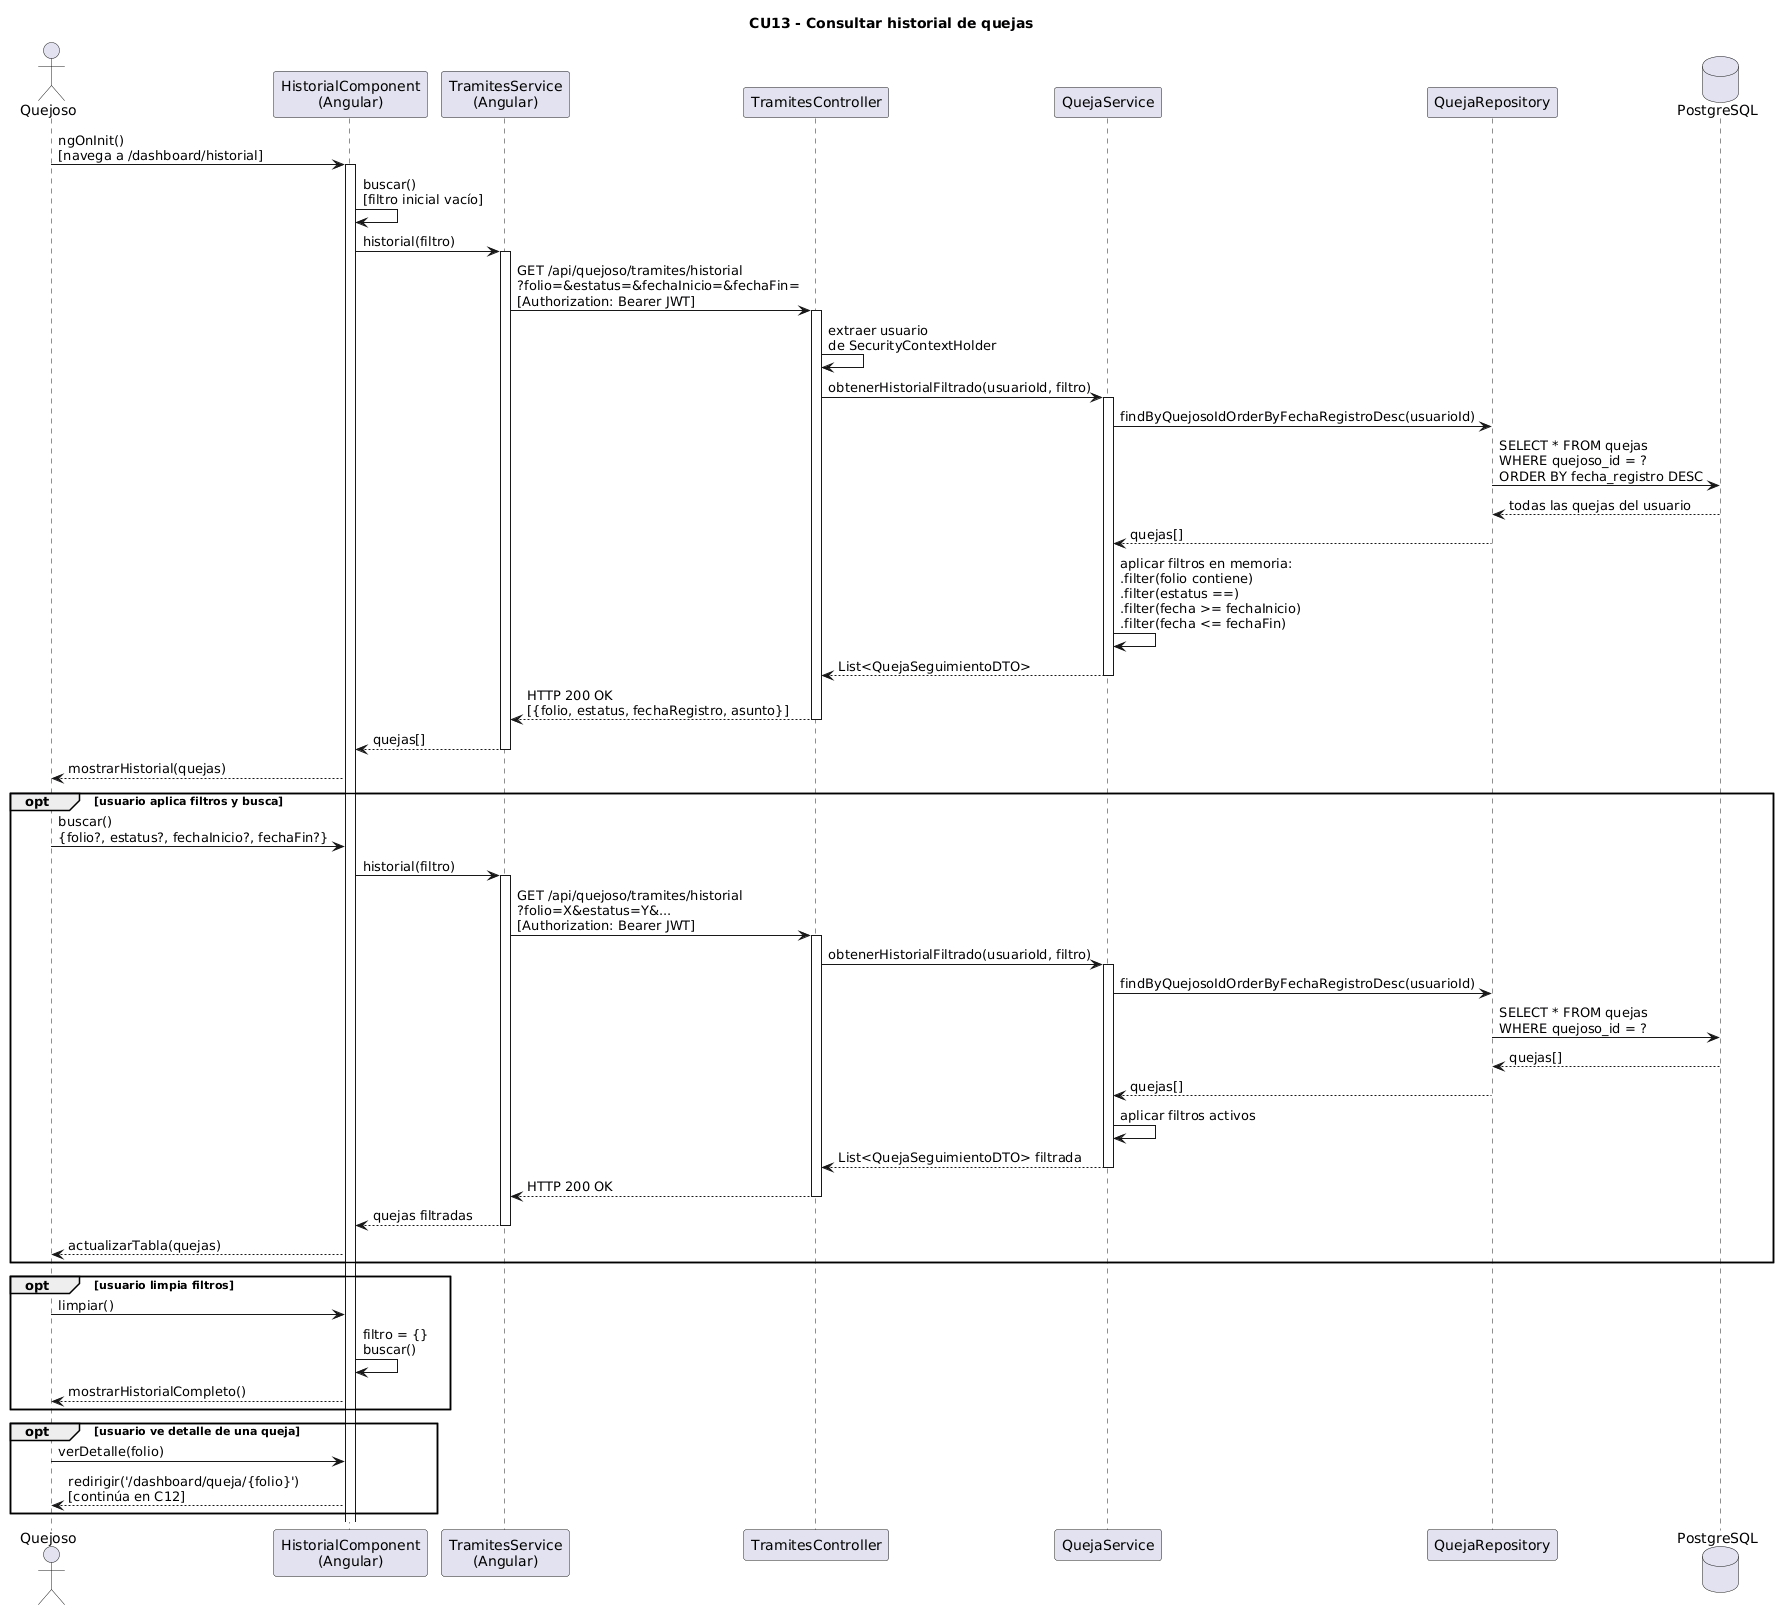
\includegraphics[width=0.90\textwidth, height=0.80\textheight, keepaspectratio]{imagenes/quejoso/D_Secuencia/CU13-HistorialQuejas.png}
        \caption{Diagrama de Secuencia CU13: Historial de Quejas}
        \label{fig:ds_cu13_historial_quejas}
    \end{figure}

    \clearpage

    % ---- CU14 ----
    \subsubsection{CU14: Levantar Queja desde Dashboard}

    Ilustra la secuencia de registro de una nueva queja para el quejoso ya autenticado. A diferencia de CU01, el flujo muestra la recuperación automática de los datos de perfil del usuario para pre-llenar el formulario, reduciendo la información que el quejoso debe capturar manualmente.

    \begin{figure}[H]
        \centering
        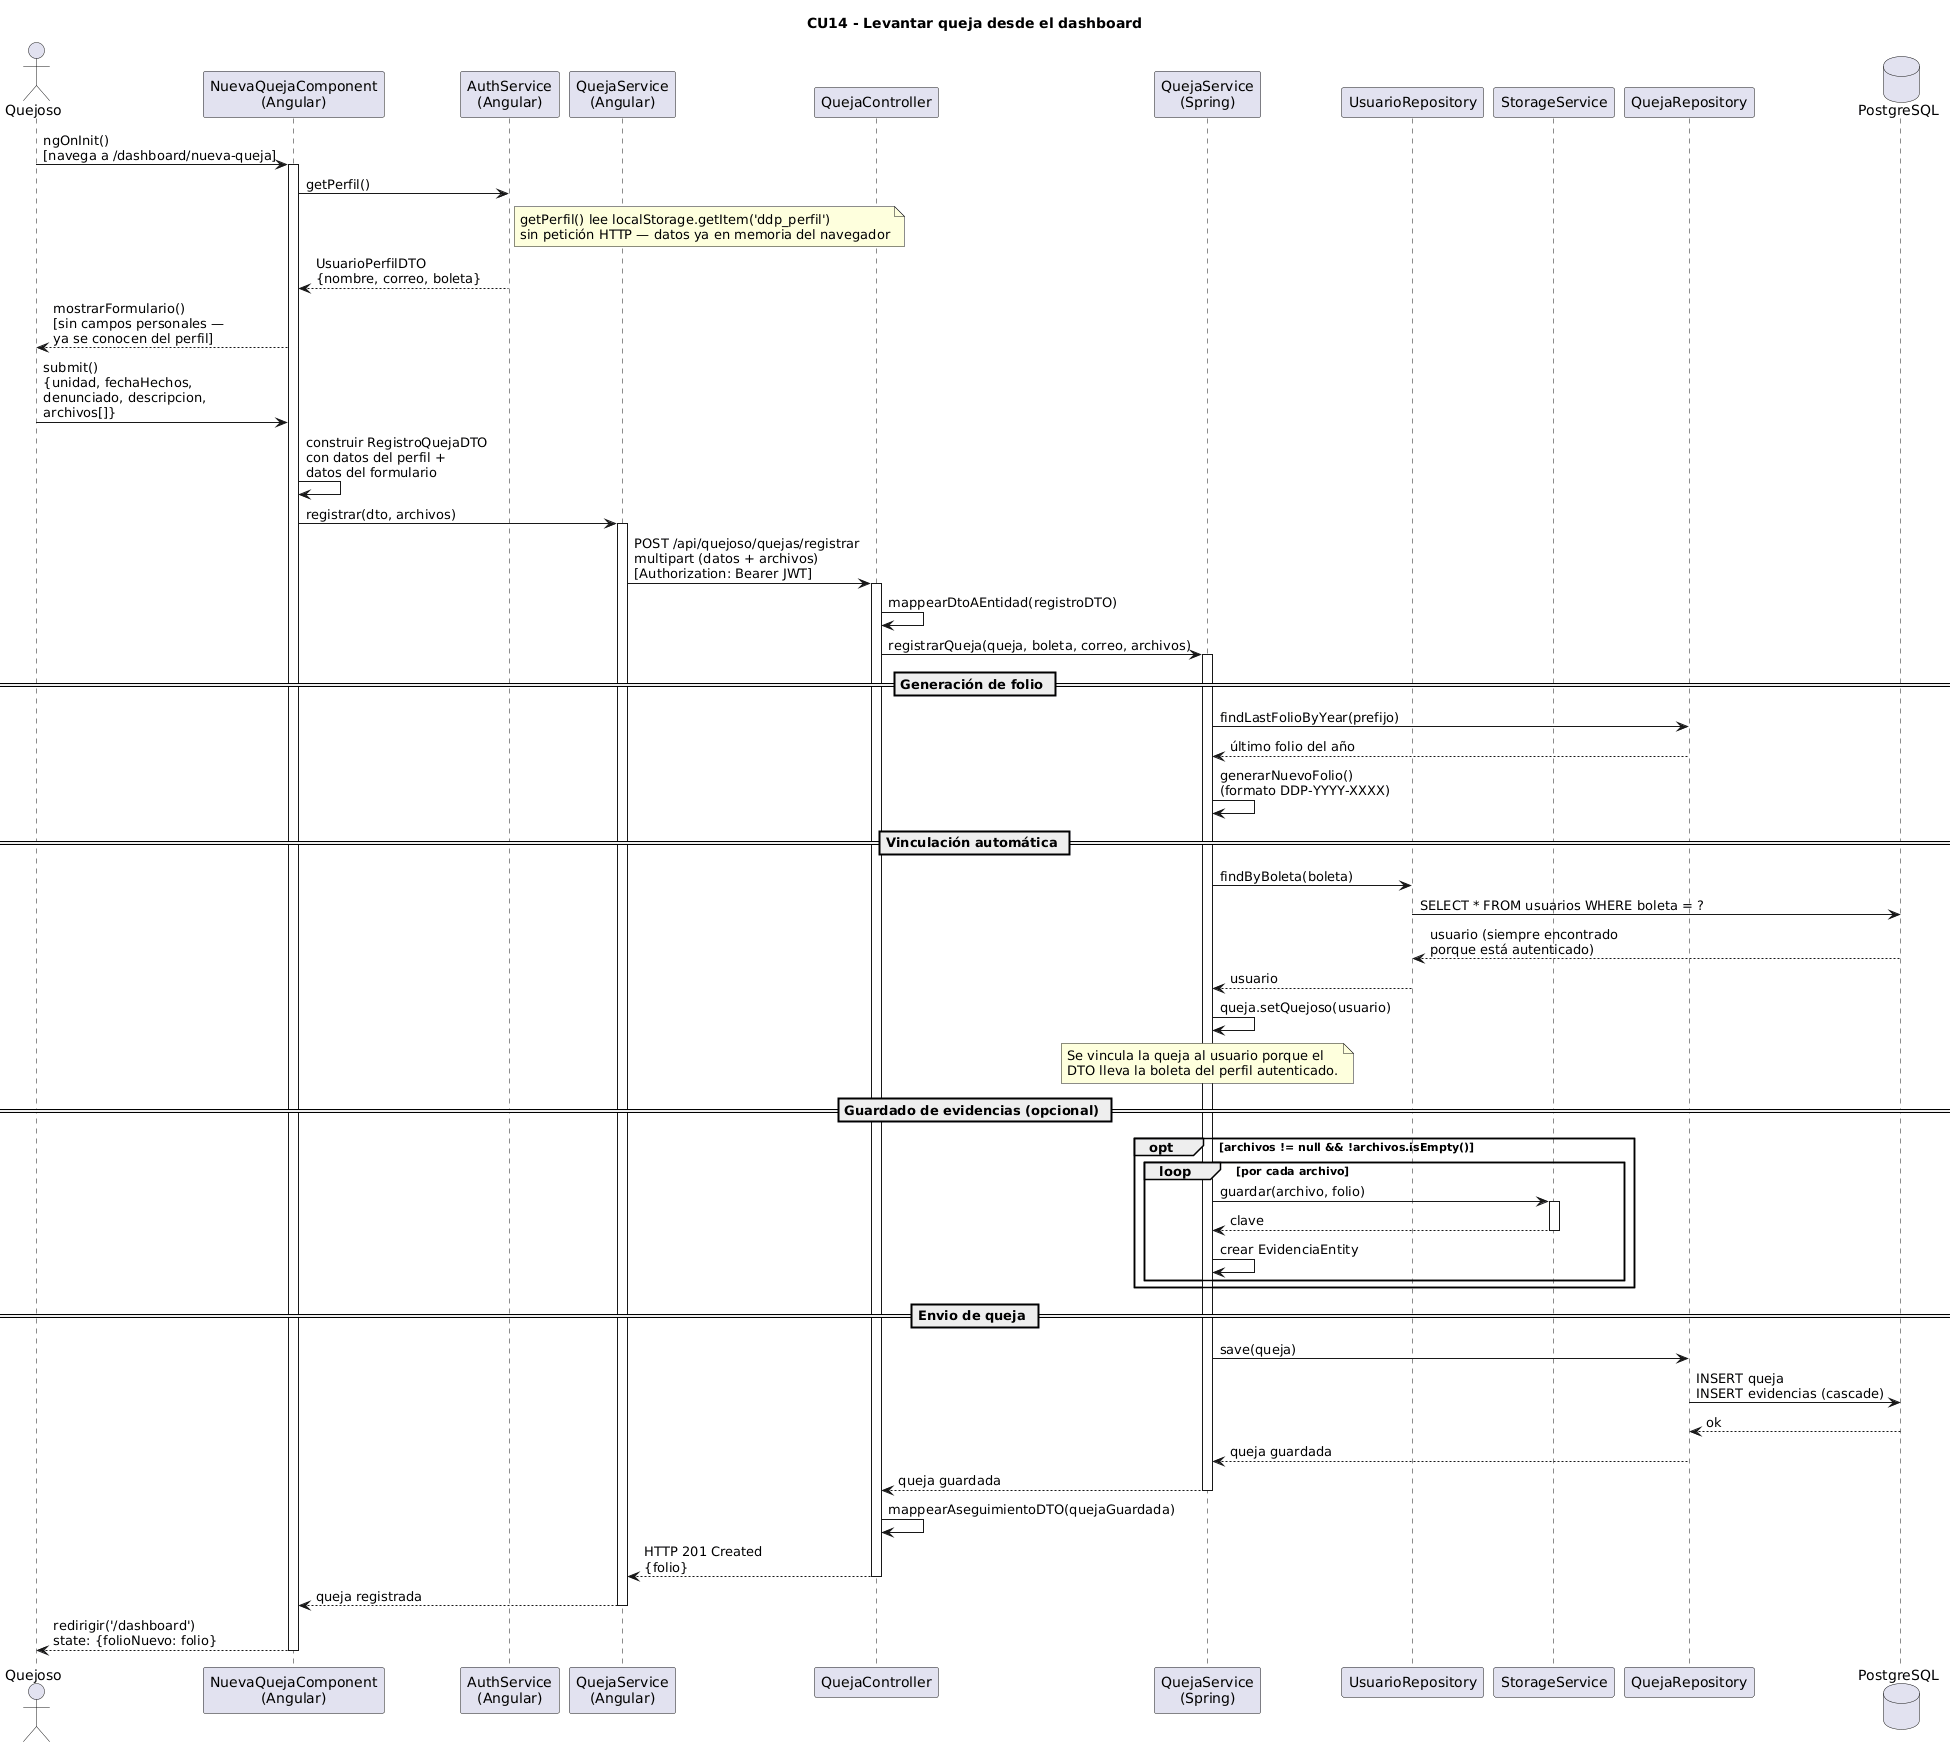
\includegraphics[width=0.90\textwidth, height=0.80\textheight, keepaspectratio]{imagenes/quejoso/D_Secuencia/CU14-LevantarQuejaDashboard.png}
        \caption{Diagrama de Secuencia CU14: Levantar Queja desde Dashboard}
        \label{fig:ds_cu14_levantar_queja_dashboard}
    \end{figure}

    \clearpage

    % ---- CU15 ----
    \subsubsection{CU15: Notificaciones}

    Describe el flujo de consulta del centro de notificaciones del quejoso. El diagrama muestra la recuperación cronológica de alertas desde el backend (cambios de estatus, requerimientos de información adicional), su presentación en la interfaz y el marcado como leídas al ser consultadas.

    \begin{figure}[H]
        \centering
        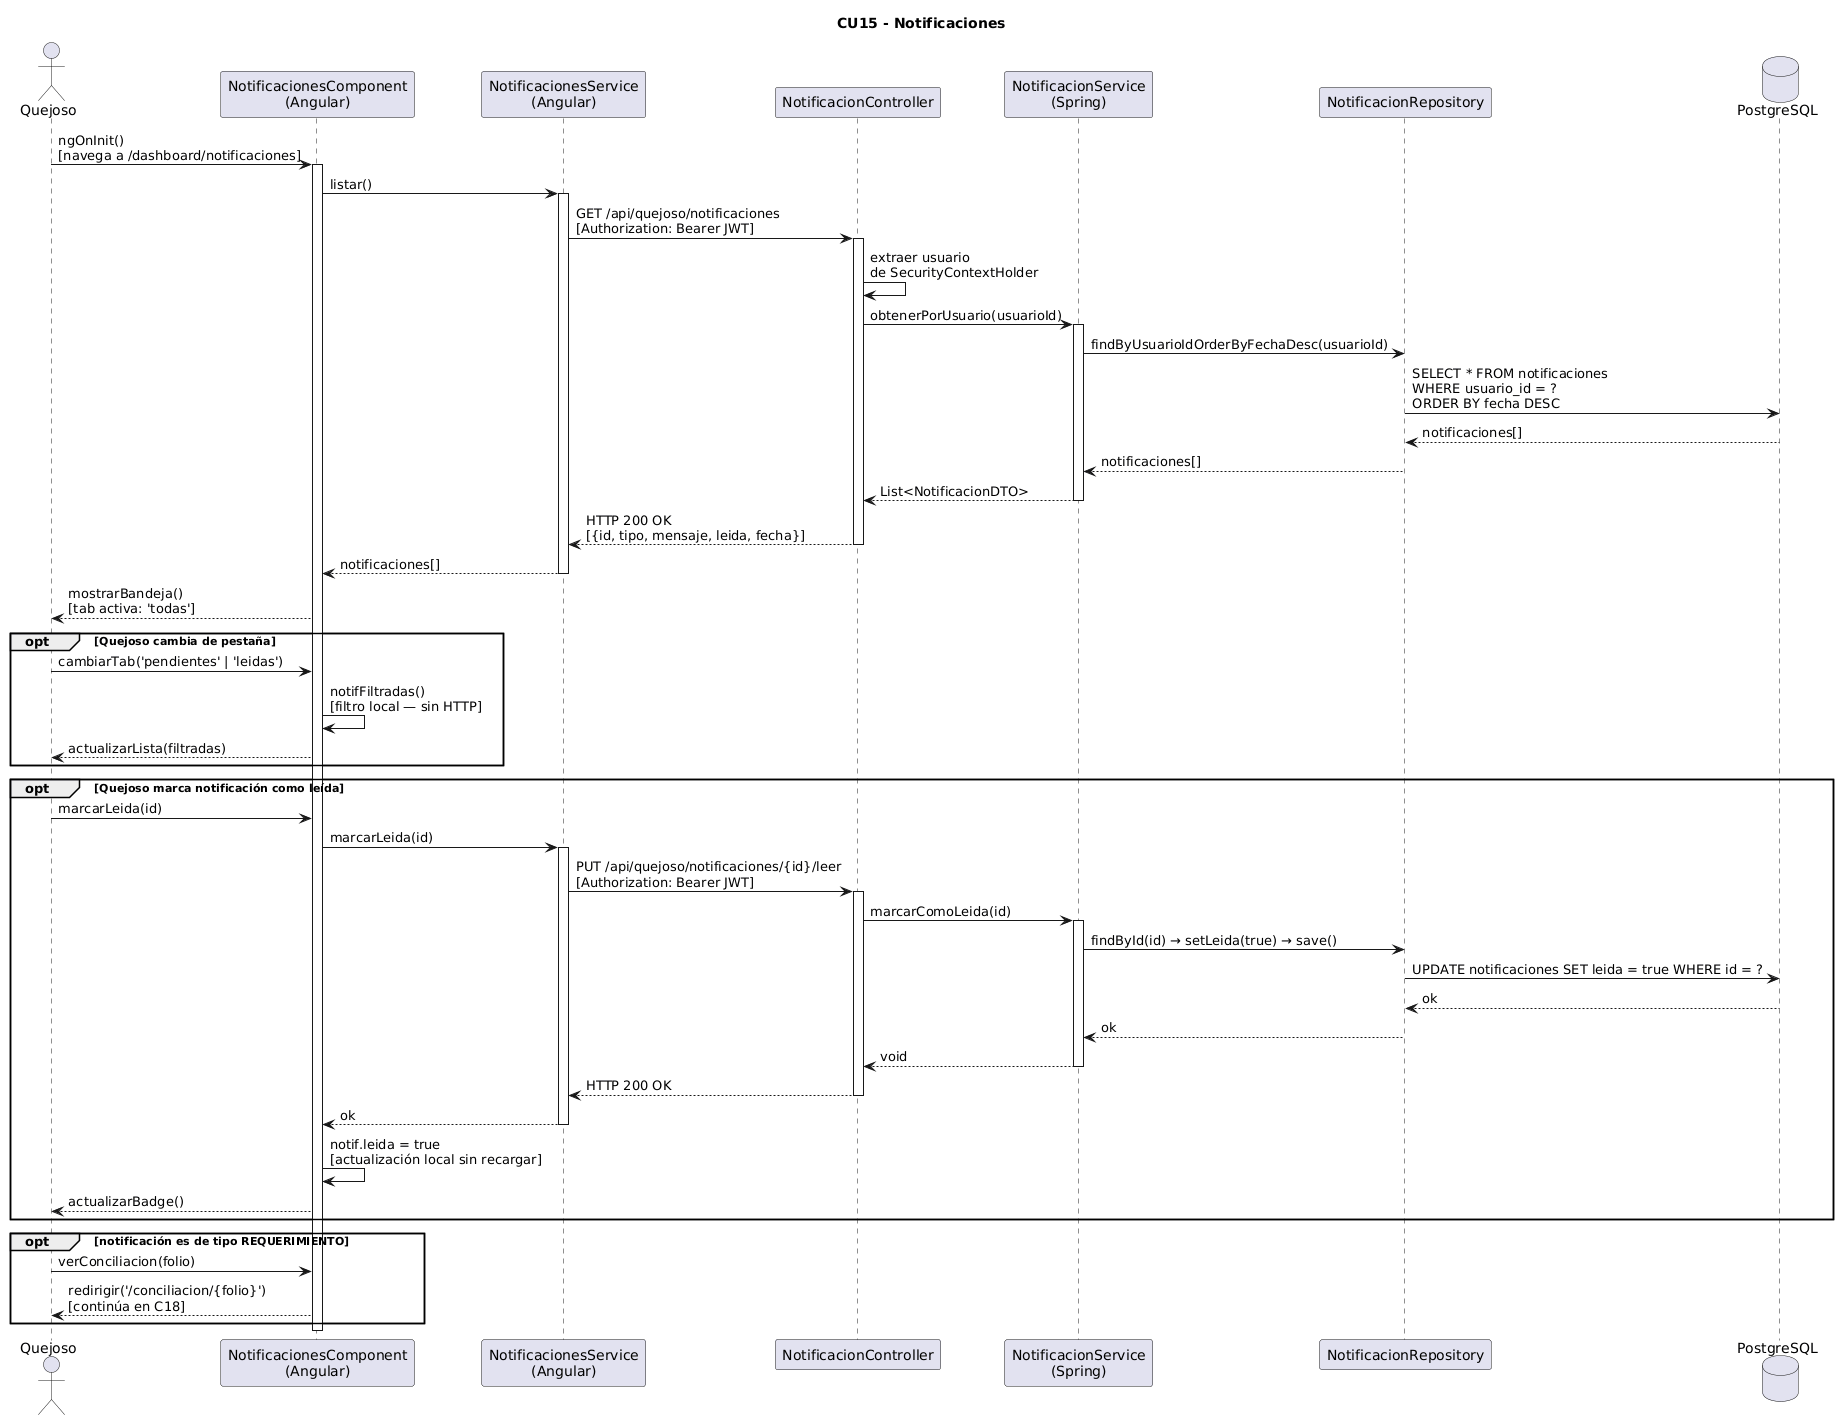
\includegraphics[width=0.90\textwidth, height=0.80\textheight, keepaspectratio]{imagenes/quejoso/D_Secuencia/CU15-Notificaciones.png}
        \caption{Diagrama de Secuencia CU15: Notificaciones}
        \label{fig:ds_cu15_notificaciones}
    \end{figure}

    \clearpage

    % ---- CU18 ----
    \subsubsection{CU18: Acuerdos de Conciliación}

    Representa la secuencia de interacción del quejoso con las propuestas de conciliación emitidas por la Defensoría. El diagrama contempla la consulta de propuestas pendientes, la presentación del detalle del acuerdo y el flujo de aceptación o rechazo, incluyendo el registro obligatorio de la justificación en caso de rechazo.

    \begin{figure}[H]
        \centering
        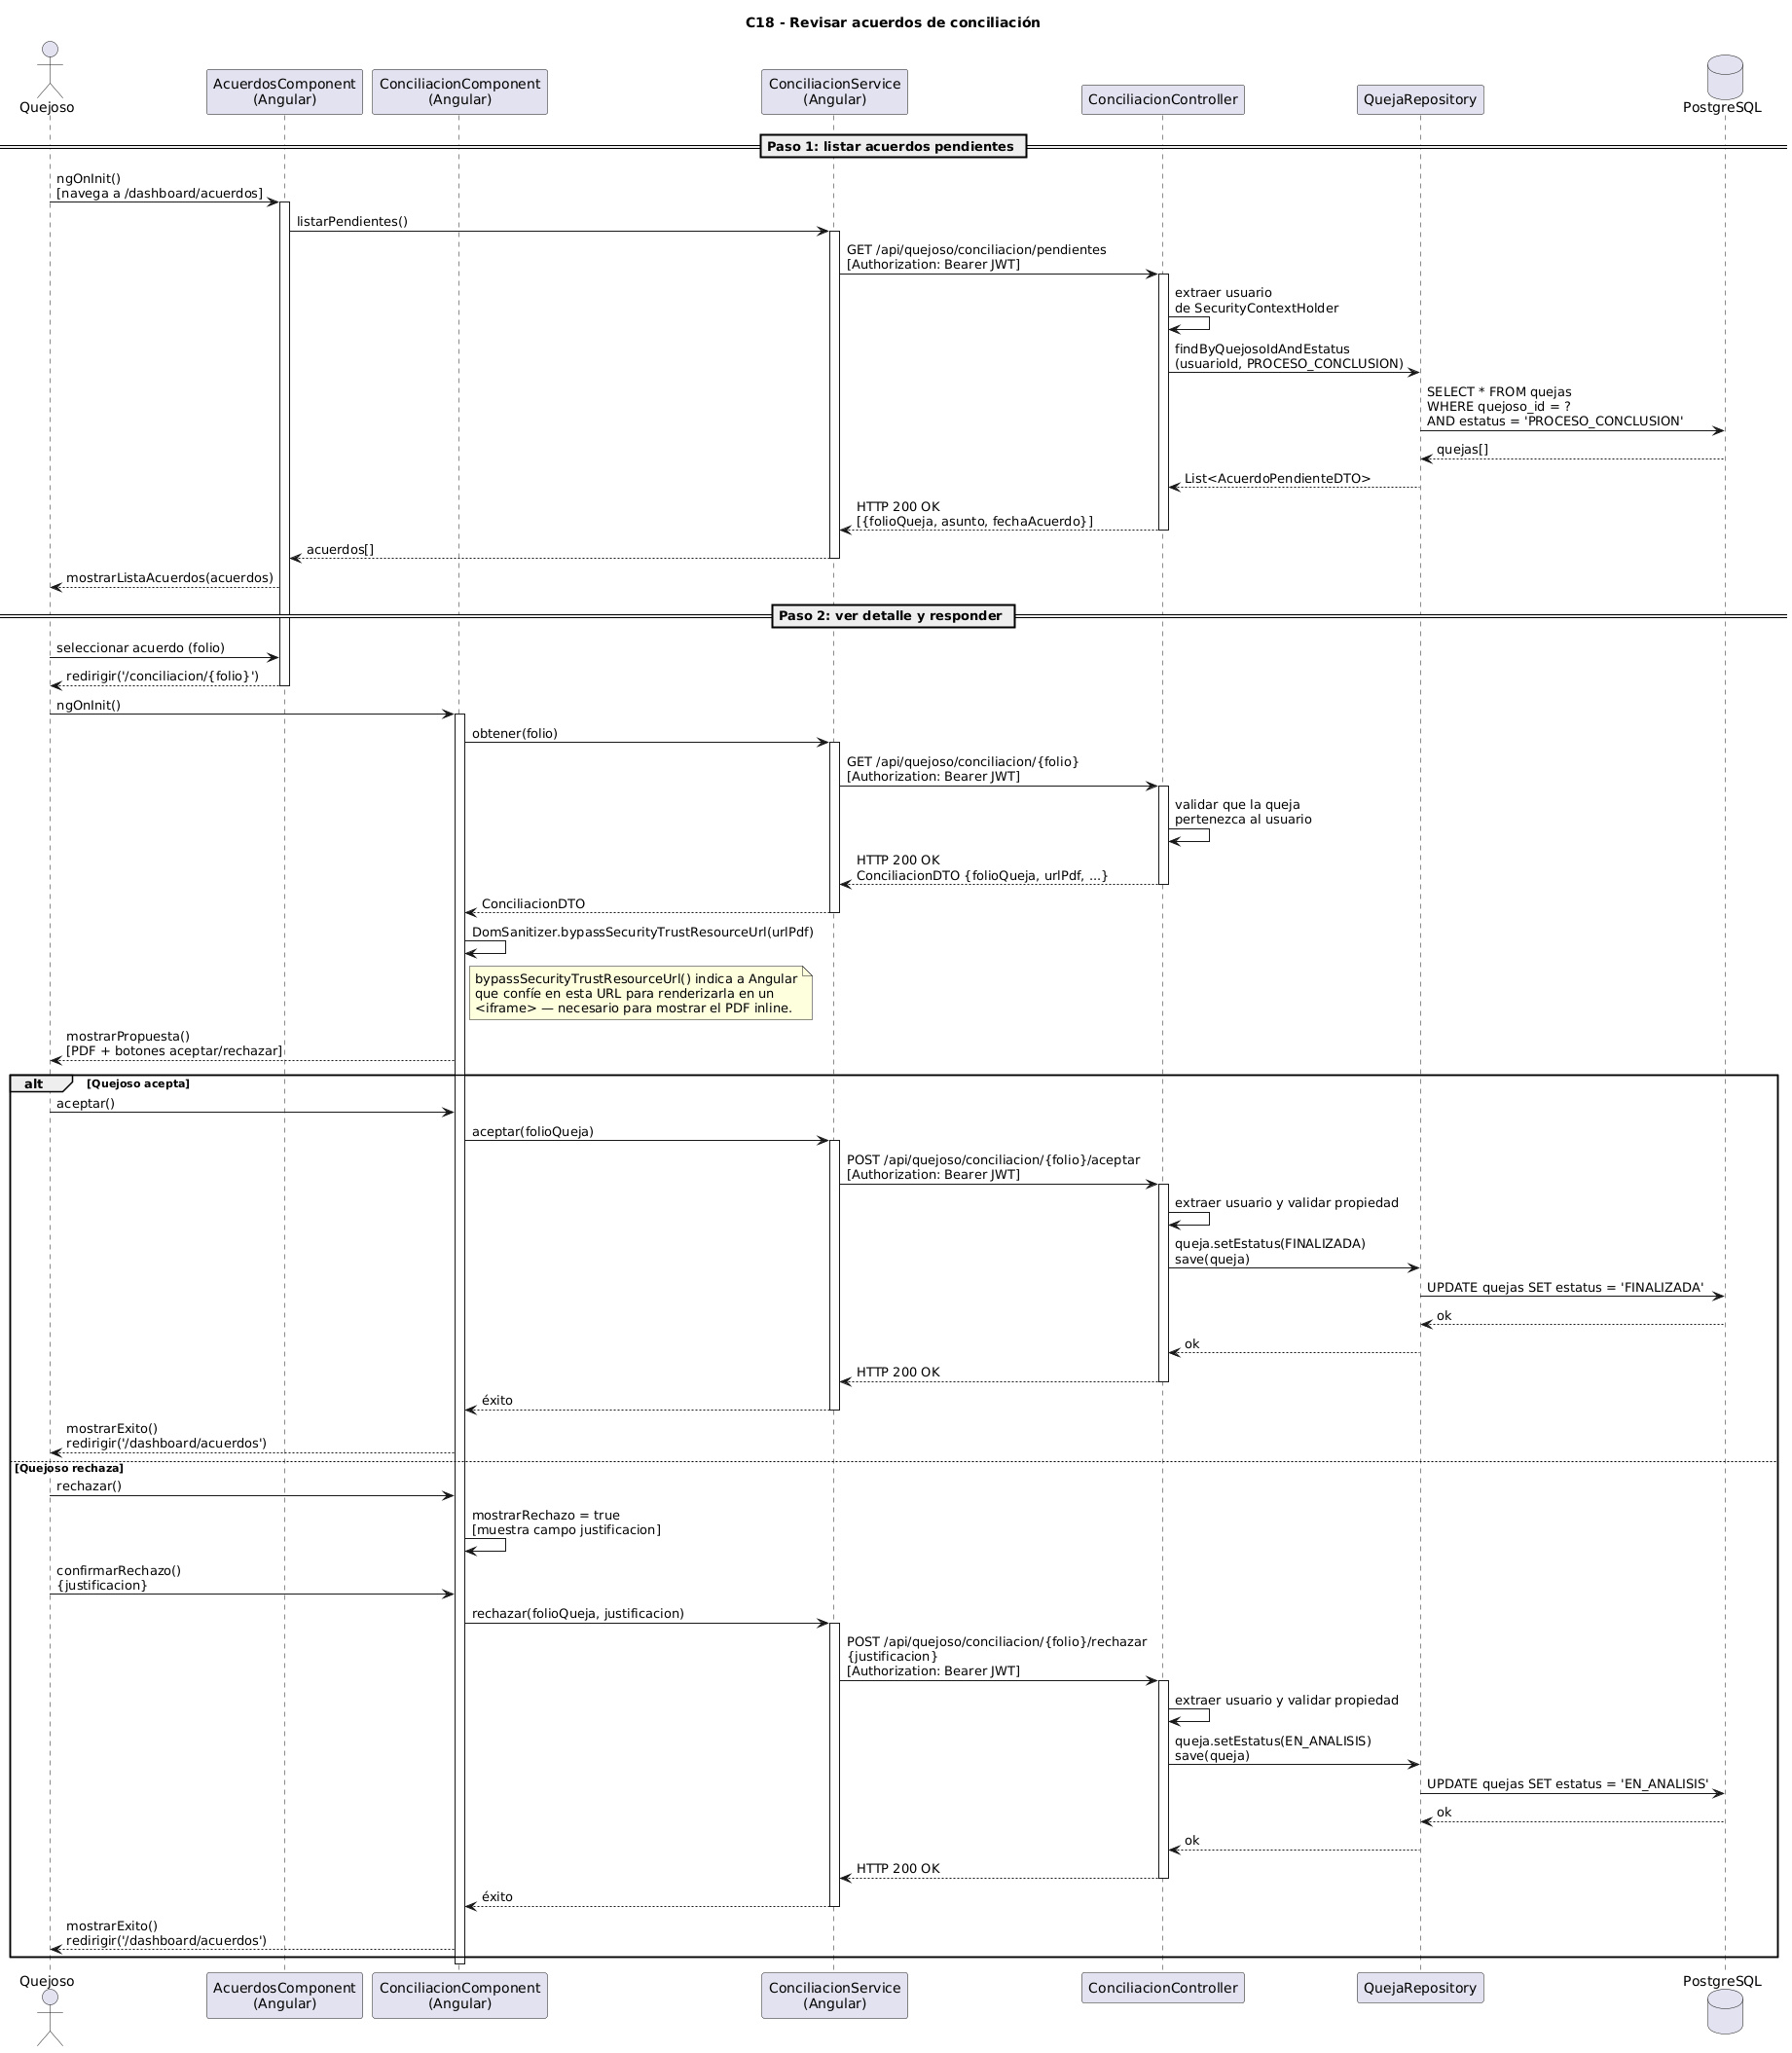
\includegraphics[width=0.90\textwidth, height=0.80\textheight, keepaspectratio]{imagenes/quejoso/D_Secuencia/CU18-AcuerdosConciliacion.png}
        \caption{Diagrama de Secuencia CU18: Acuerdos de Conciliación}
        \label{fig:ds_cu18_acuerdos_conciliacion}
    \end{figure}

    \clearpage

    % ---- CU19 ----
    \subsubsection{CU19: Ver Perfil}

    Ilustra la secuencia de consulta y actualización del perfil del quejoso autenticado. El flujo muestra la recuperación de los datos personales almacenados (nombre, correo, teléfono y datos del tutor si aplica), la edición de los campos de contacto y la persistencia de los cambios en la base de datos.

    \begin{figure}[H]
        \centering
        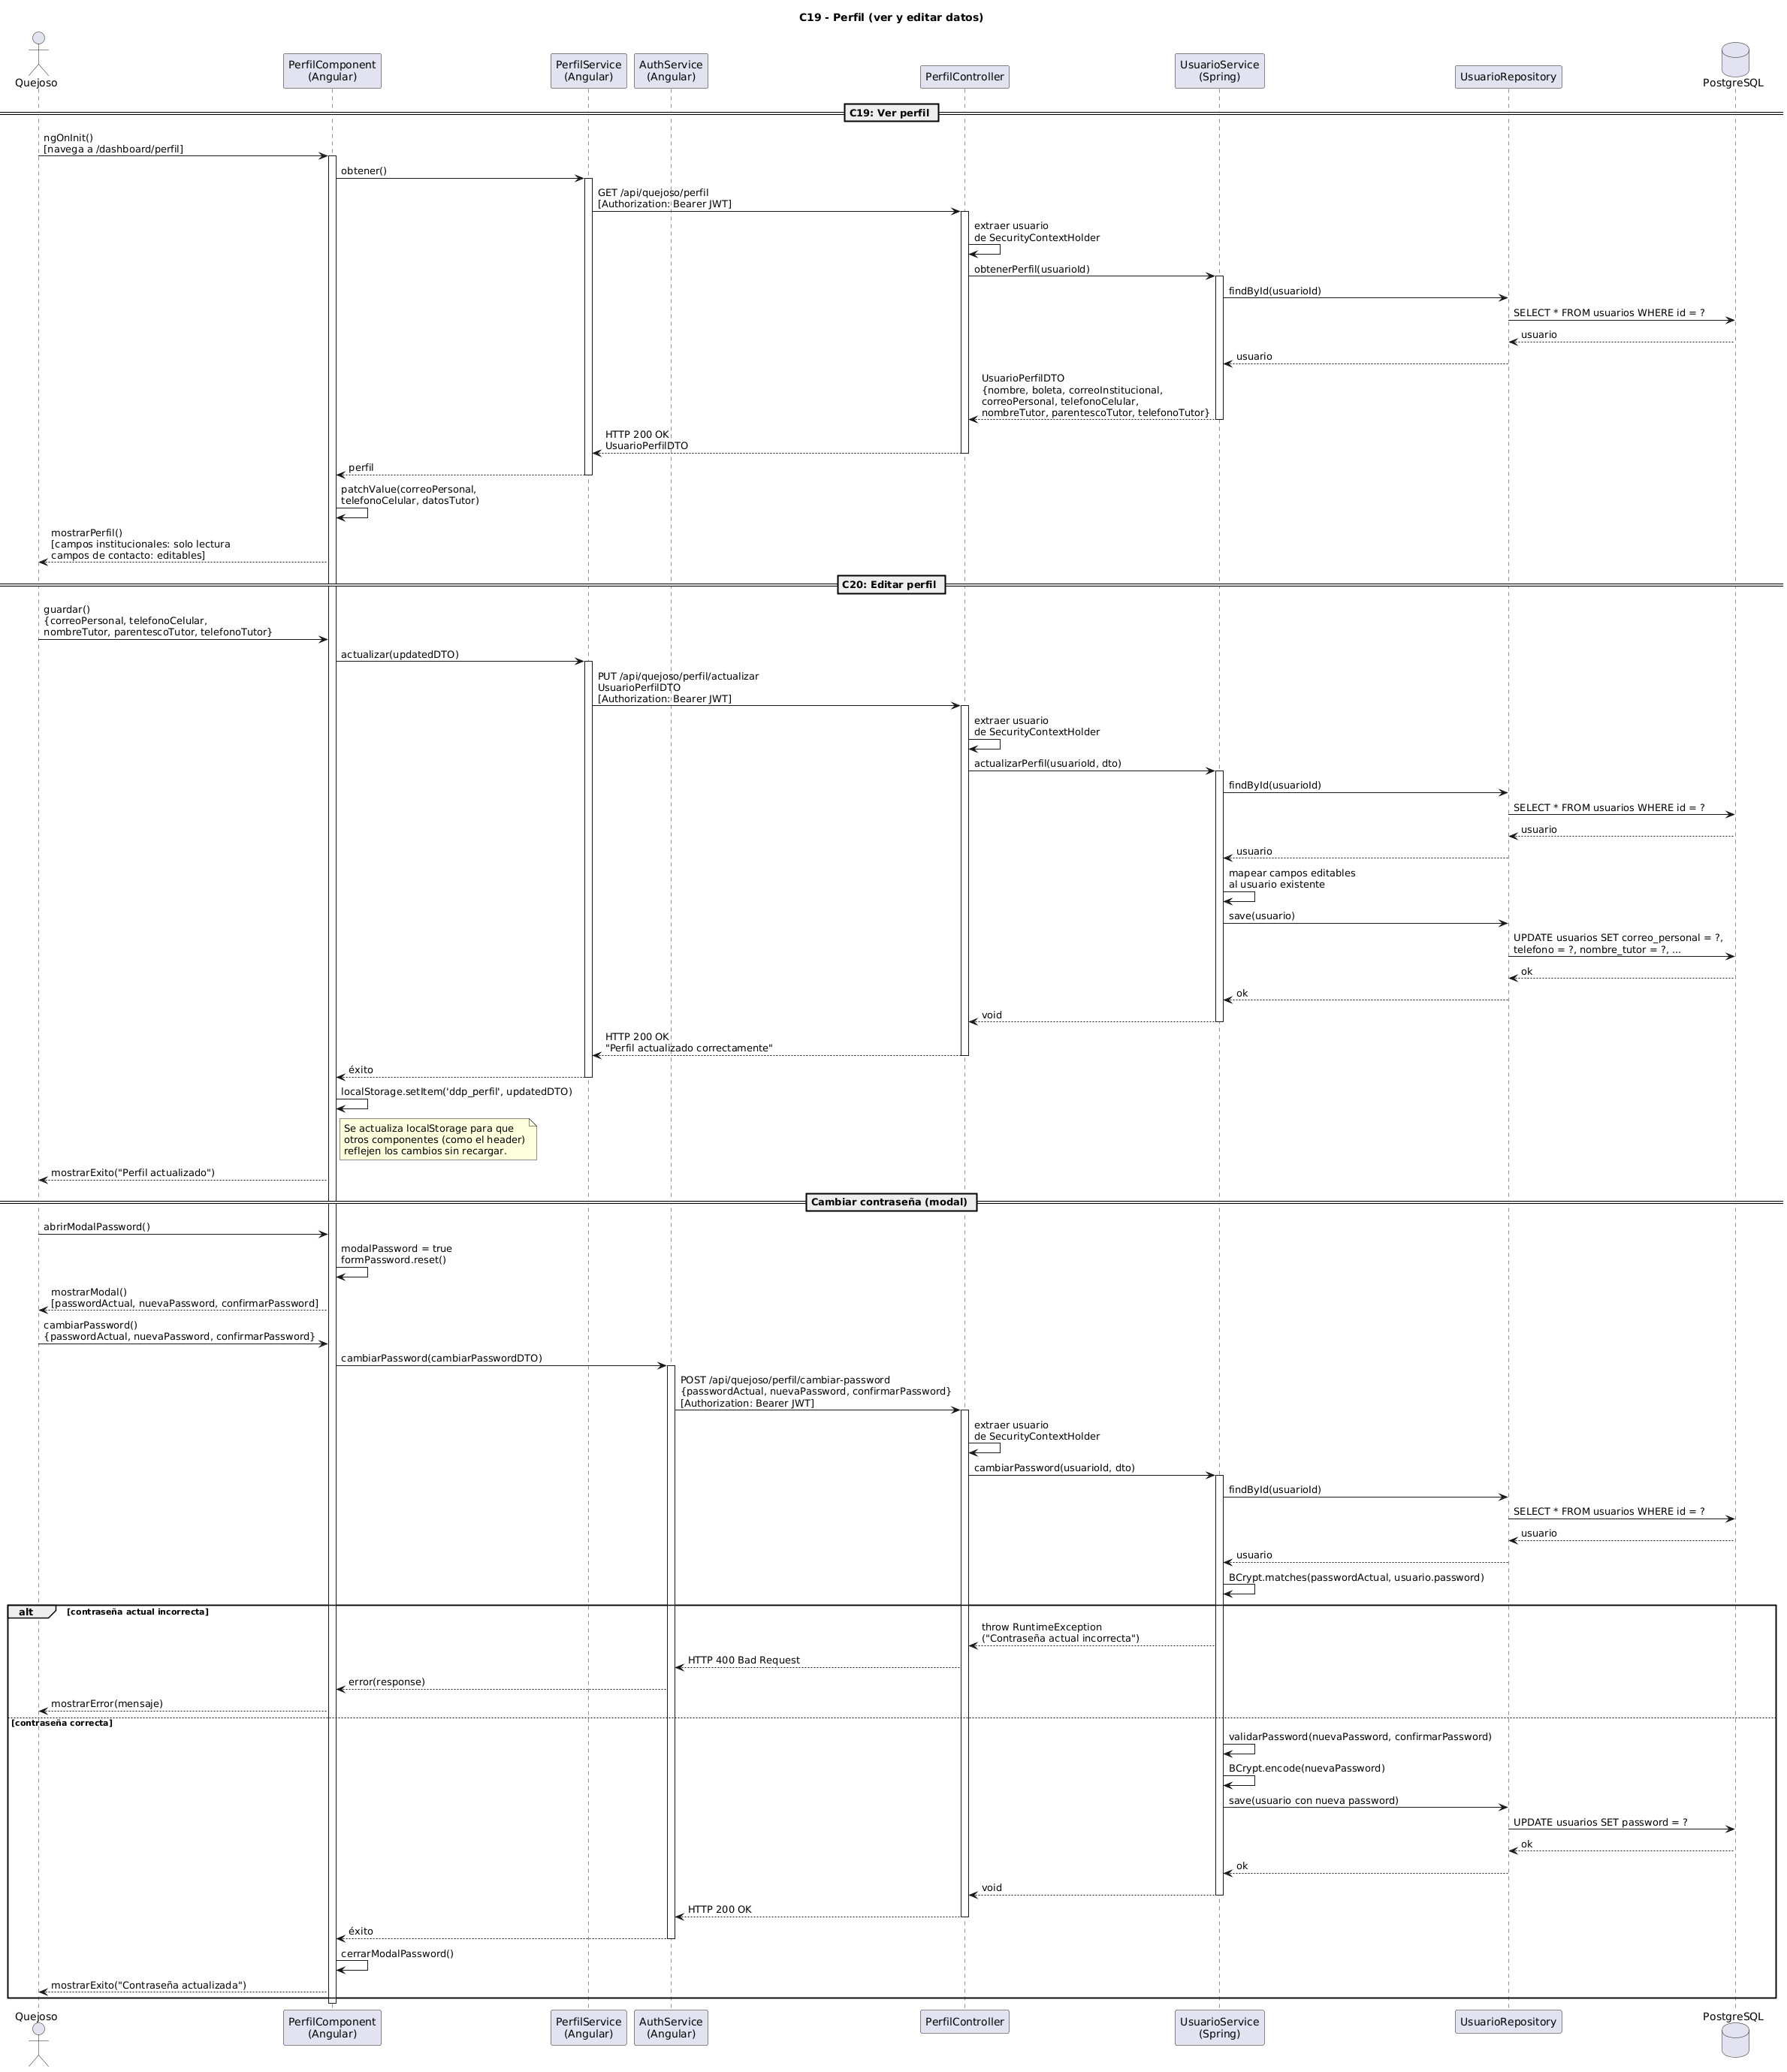
\includegraphics[width=0.90\textwidth, height=0.80\textheight, keepaspectratio]{imagenes/quejoso/D_Secuencia/CU19-VerPerfil.png}
        \caption{Diagrama de Secuencia CU19: Ver Perfil}
        \label{fig:ds_cu19_ver_perfil}
    \end{figure}

\end{document}
